% TPA-12 presentation (Beamer, 16:9), about 10 minutes.
\documentclass[aspectratio=169,10pt]{beamer}
\usetheme{Madrid}
\definecolor{iitblue}{RGB}{22,50,74}
\definecolor{accent}{RGB}{47,111,159}
\definecolor{warm}{RGB}{181,101,29}
\definecolor{soft}{RGB}{238,243,248}
\setbeamercolor{structure}{fg=accent}
\setbeamercolor{palette primary}{bg=iitblue,fg=white}
\setbeamercolor{palette secondary}{bg=accent,fg=white}
\setbeamercolor{palette tertiary}{bg=iitblue,fg=white}
\setbeamercolor{frametitle}{bg=iitblue,fg=white}
\setbeamercolor{block title}{bg=accent,fg=white}
\setbeamercolor{block body}{bg=soft}
\setbeamertemplate{navigation symbols}{}
\setbeamertemplate{blocks}[rounded][shadow=false]
\setbeamertemplate{itemize items}[circle]
\setbeamertemplate{enumerate items}[default]
\setlength{\leftmargini}{1.2em}
\usepackage{amsmath,amssymb}
\usepackage{booktabs}
\usepackage{array}
\usepackage{graphicx}
\graphicspath{{../final/figures/}{../figures/}}
\newcommand{\R}{\mathbf{R}}
\newcommand{\tv}{\mathbf{t}}
\newcommand{\K}{\mathbf{K}}
\newcommand{\X}{\mathbf{X}}
\newcommand{\x}{\mathbf{x}}
\newcommand{\n}{\mathbf{n}}
\newcommand{\p}{\mathbf{p}}
\newcommand{\head}[1]{{\usebeamercolor[fg]{structure}\textbf{#1}}}
\newcommand{\cit}[1]{{\scriptsize\textcolor{black!55}{[#1]}}}

\title[TPA-12: Change in 3D pose of small objects]{Compute change in pose (3D) of a small object}
\author[Chiramana, Chanduluri]{Sai Svanik Chiramana (ME23B195) \and Sathwik Chanduluri (ME23B238)}
\institute[IIT Madras]{Group 3 \textbullet\ CS6350 Computer Vision, TPA-12 \textbullet\ IIT Madras}
\date{}

\begin{document}

% ------------------------------------------------------------------ 1 title
\begin{frame}[plain]
  \centering
  \vspace*{0.2cm}
  
\includegraphics[height=1.6cm]{iitm_logo.png}\par\vspace{0.4cm}
  {\usebeamercolor[fg]{structure}\large\bfseries Compute change in pose (3D) of a small object (coin, key, mobile phone, purse, clock, plate, checkerboard etc.) with very high accuracy from two successive views (arbitrary) of the same object (objects can have a near planar surface)\par}
  \vspace{0.6cm}
  {\normalsize Sai Svanik Chiramana (ME23B195) \qquad Sathwik Chanduluri (ME23B238)\par}
  \vspace{0.3cm}
  {\normalsize\bfseries Group 3\par}
  \vspace{0.3cm}
  {\small CS6350 Computer Vision \textbullet\ TPA-12 \textbullet\ Prof.\ Sukhendu Das \textbullet\ Indian Institute of Technology Madras\par}
\end{frame}

% ------------------------------------------------------------------ 2 problem
\begin{frame}{Problem statement}
  \begin{columns}[c]
    \begin{column}{0.53\textwidth}
      \head{What the task asks.} Given two RGB images of the same small object taken from arbitrary viewpoints, compute the change in its 3D pose with high accuracy. The object may be nearly planar.\\[6pt]
      \head{Input.} Only the two images: no camera intrinsics, no object mask and no object name.\\[6pt]
      \head{Output.}
      \begin{itemize}
        \item the relative rotation matrix $\R$
        \item the relative translation vector $\tv$ --- its direction; the length needs the object's size
        \item reprojection error metrics indicating the accuracy
      \end{itemize}
      \vspace{4pt}
      \[\X_2=\R\,\X_1+\tv,\qquad \R^\top\R=I,\ \det\R=1\]
    \end{column}
    \begin{column}{0.43\textwidth}
      \begin{block}{Why it is difficult}
        \begin{itemize}
          \item \textbf{Small object:} most matches lie on the background and describe its motion.
          \item \textbf{Weak texture:} phone backs, metal keys and watch faces give few features.
          \item \textbf{Near-planar:} a plane admits two valid poses; $E$ becomes ill-conditioned.
          \item \textbf{Large viewpoint change:} local appearance changes beyond $30^\circ$.
          \item \textbf{Nothing else given:} focal length and object location must be estimated.
        \end{itemize}
      \end{block}
    \end{column}
  \end{columns}
\end{frame}

% ------------------------------------------------------------------ 3 pipeline
\begin{frame}{Proposed solution: the two-image pipeline}
  \centering
  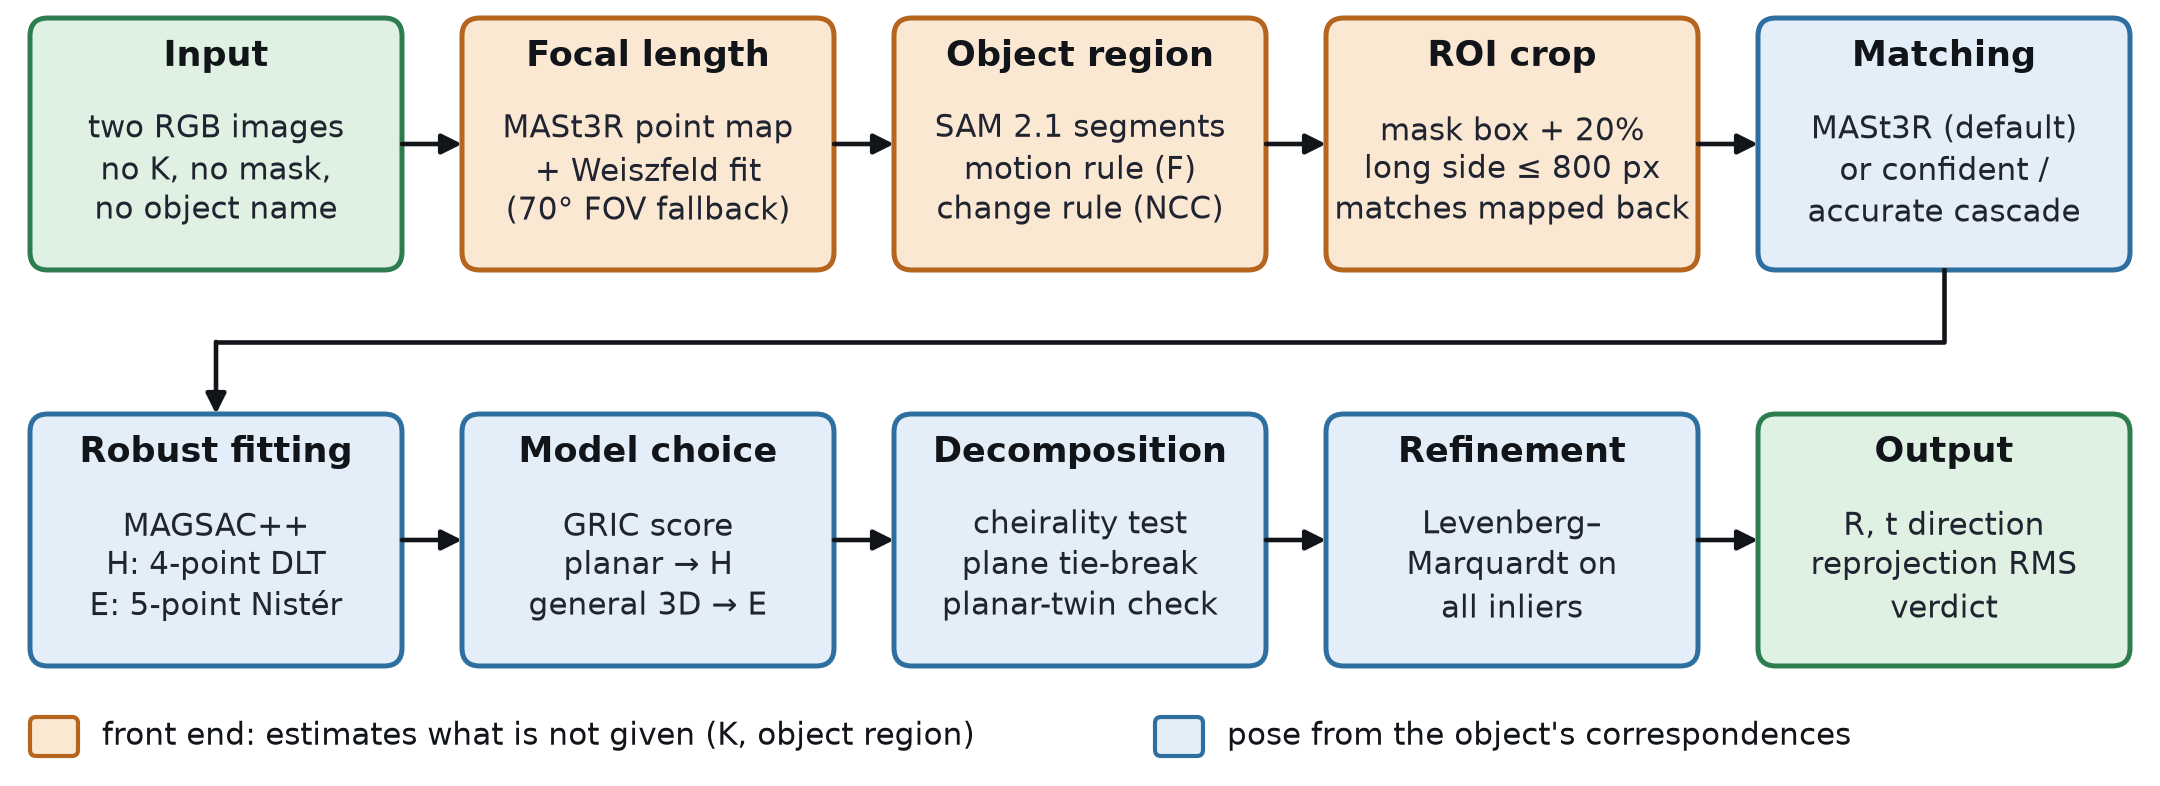
\includegraphics[width=\textwidth]{pipeline.png}\par
  \vspace{8pt}
  \begin{columns}[t]
    \begin{column}{0.48\textwidth}
      \small\textcolor{warm}{\textbf{Front end}} --- estimates what is not given: the focal length (from a predicted 3D point map) and the object region (the segment that moved relative to the background).
    \end{column}
    \begin{column}{0.48\textwidth}
      \small\textcolor{accent}{\textbf{Pose estimation}} --- correspondences on the object, robust fitting of $H$ and $E$, model choice, decomposition and refinement; outputs $\R$, the direction of $\tv$ and the reprojection error.
    \end{column}
  \end{columns}
\end{frame}

% ------------------------------------------------------------------ 4 focal
\begin{frame}{Step 1 --- Focal length from the images}
  \begin{columns}[c]
    \begin{column}{0.5\textwidth}
      \head{Why.} The focal length turns pixels into viewing rays; a 10\% error costs about 6 AUC@10 points, and no calibration is given.\\[8pt]
      \head{How.}
      \begin{itemize}
        \item MASt3R (Matching And Stereo 3D Reconstruction)~\cit{3} predicts a 3D point for every pixel of image 1.
        \item With the principal point at the centre, each pixel votes for one $f$.
        \item Weiszfeld's robust fit~\cit{2} combines the votes; repeated with the images swapped and averaged.
      \end{itemize}
      \vspace{4pt}
      \head{Result.} Median focal error 6\%.
    \end{column}
    \begin{column}{0.46\textwidth}
      \begin{block}{Equations}
        Pinhole projection and pixel ray~\cit{1}:
        \[\lambda\,(u,v,1)^\top=\K\X,\qquad \x=\K^{-1}(u,v,1)^\top\]
        Vote of pixel $i$:
        \[(u_i-c_x,\ v_i-c_y)\approx f\,(X_i/Z_i,\ Y_i/Z_i)\]
        Robust combination:
        \[f^\star=\arg\min_f\sum_i\big\|\p_i-\mathbf{c}-f\,\mathbf{q}_i\big\|\]
      \end{block}
    \end{column}
  \end{columns}
\end{frame}

% ------------------------------------------------------------------ 5 SAM
\begin{frame}{Step 2a --- Candidate objects with SAM 2.1}
  \begin{columns}[c]
    \begin{column}{0.5\textwidth}
      \head{Why.} A small object is outnumbered by the background, whose matches describe the camera's motion. Its pixels must be found without a box or a name.\\[8pt]
      \head{SAM 2.1 (Segment Anything Model)~\cit{5}.} A Hiera (hierarchical vision transformer)~\cit{6} encoder reads the image once; a light two-way decoder returns the mask under each prompt, with no class name needed.\\[8pt]
      \head{Our use.} A $12\times12$ grid of point prompts; duplicates merged, border-touching and wrongly sized segments dropped.
    \end{column}
    \begin{column}{0.46\textwidth}
      \begin{block}{Equations}
        Duplicate masks are merged when (Intersection over Union)
        \[\mathrm{IoU}=\frac{|A\cap B|}{|A\cup B|}>0.8\]
        Candidates are ranked by
        \[\text{score}=\text{area}\times\big(0.25+\text{centrality}\big)\]
        \[\text{centrality}=1-\frac{\|\mathbf{c}-(\tfrac12,\tfrac12)\|}{\sqrt{1/2}}\]
      \end{block}
    \end{column}
  \end{columns}
\end{frame}

% ------------------------------------------------------------------ 6 moved object
\begin{frame}{Step 2b --- Which candidate moved?}
  \begin{columns}[c]
    \begin{column}{0.5\textwidth}
      \head{Idea.} If only the camera moves, the background shifts consistently; a hand-moved object breaks that pattern.\\[8pt]
      \head{Motion rule.} Fit the background's fundamental matrix $F$ with MAGSAC++ (Marginalizing Sample Consensus)~\cit{7}; a candidate whose matches mostly break it has moved.\\[8pt]
      \head{Change rule~\cit{8}.} For shiny or dark objects: undo the background's motion by warping, then check whether the region still aligns.\\[8pt]
      \head{Decision.} Largest moved segment = object; nothing moved $\Rightarrow$ static scene, whole images.
    \end{column}
    \begin{column}{0.46\textwidth}
      \begin{block}{Equations}
        Static points obey
        \[\p_2^\top F\,\p_1=0\]
        Sampson distance of a match~\cit{1}:
        \[d_S^2=\frac{(\p_2^\top F\p_1)^2}{\|(F\p_1)_{1:2}\|^2+\|(F^\top\p_2)_{1:2}\|^2}\]
        Normalised cross-correlation (NCC)~\cit{9}:
        \[\mathrm{NCC}=\frac{\sum(a-\bar a)(b-\bar b)}{\sqrt{\sum(a-\bar a)^2\sum(b-\bar b)^2}}\]
      \end{block}
    \end{column}
  \end{columns}
\end{frame}

% ------------------------------------------------------------------ 7 matching
\begin{frame}{Step 3 --- Crop and correspondences with MASt3R}
  \begin{columns}[c]
    \begin{column}{0.5\textwidth}
      \small\head{Crop.} Object box $+20\%$, at most 800\,px; matches mapped back, so $\K$ is unchanged.\\[5pt]
      \head{MASt3R (Matching And Stereo 3D Reconstruction)~\cit{3}.} Built on DUSt3R (Dense and Unconstrained Stereo 3D Reconstruction)~\cit{4}: a ViT (Vision Transformer) encoder with cross-attending decoders predicts a 3D point and a descriptor per pixel.\\[5pt]
      \head{Alternatives.} SIFT (Scale-Invariant Feature Transform)~\cit{10}, XFeat (Accelerated Features)~\cit{11} + LightGlue~\cit{12}, LoFTR (Local Feature TRansformer)~\cit{13}.\\[5pt]
      \head{Cascades.} \texttt{accurate}: XFeat+LightGlue $\rightarrow$ outline $\rightarrow$ SIFT $\rightarrow$ LoFTR, taking the first with enough inliers. \texttt{confident}: XFeat+LightGlue $\rightarrow$ SIFT $\rightarrow$ outline $\rightarrow$ MASt3R, taking a stage only if a learned classifier predicts $P(e<10^\circ)\ge0.45$.
    \end{column}
    \begin{column}{0.46\textwidth}
      \begin{block}{Equations}
        Crop back to image coordinates:
        \[\p_{\text{full}}=\p_{\text{crop}}/s+\mathbf{o}\]
        Mutual nearest neighbours:
        \[j=\arg\max_k\,\mathbf{d}^{1\top}_i\mathbf{d}^2_k,\quad i=\arg\max_l\,\mathbf{d}^{2\top}_j\mathbf{d}^1_l\]
        Confidence-weighted training loss~\cit{4}:
        \[\mathcal{L}=\sum_i C_i\,\|\X_i-\hat\X_i\|-\alpha\log C_i\]
      \end{block}
    \end{column}
  \end{columns}
\end{frame}

% ------------------------------------------------------------------ 8 H and E
\begin{frame}{Step 4 --- Robust fitting of $H$ and $E$}
  \begin{columns}[c]
    \begin{column}{0.5\textwidth}
      \head{Two models~\cit{1}.} The homography $H$ is exact for a flat object, the essential matrix $E$ holds for any rigid object; both are fitted because the shape is unknown.\\[8pt]
      \head{MAGSAC++ (Marginalizing Sample Consensus)~\cit{7}.} Like RANSAC (Random Sample Consensus)~\cit{15}, it fits models to random minimal samples (4 matches for $H$, 5 for $E$ via Nist\'er's solver~\cit{14}) and keeps the best supported; it averages over noise levels instead of using one inlier threshold.
    \end{column}
    \begin{column}{0.46\textwidth}
      \begin{block}{Equations}
        Plane-induced homography:
        \[\p_2\simeq H\p_1,\quad H=\K_2\Big(\R+\frac{\tv\,\n^\top}{d}\Big)\K_1^{-1}\]
        Epipolar constraint:
        \[\x_2^\top E\,\x_1=0,\qquad E=[\tv]_\times\R\]
        Samples needed:
        \[N=\frac{\log(1-p)}{\log(1-w^{s})}\]
      \end{block}
    \end{column}
  \end{columns}
\end{frame}

% ------------------------------------------------------------------ 9 GRIC + decomposition
\begin{frame}{Step 5 --- Model choice (GRIC) and decomposition}
  \begin{columns}[c]
    \begin{column}{0.5\textwidth}
      \head{Model choice.} $E$ always fits at least as well as $H$; GRIC (Geometric Robust Information Criterion)~\cit{16} penalises its extra freedom, so $E$ wins only if clearly better (GRIC 44.9 vs $H$ 29.9, $E$ 44.3 AUC@10).\\[8pt]
      \head{Decomposition~\cit{1,17}.} Keep the candidate with points in front of both cameras; for a plane, off-plane matches pick between its two valid poses.\\[8pt]
      \head{Planar-twin check.} Corrects $E$ on nearly flat objects (+1--3 AUC@10).
    \end{column}
    \begin{column}{0.46\textwidth}
      \begin{block}{Equations}
        \small
        Geometric robust information criterion:
        \[\mathrm{GRIC}=\sum_i\rho\Big(\frac{e_i^2}{\sigma^2}\Big)+\lambda_1d\,n+\lambda_2k\]
        $H$: $d=2,\ k=8$; \quad $E$: $d=3,\ k=5$.\\[4pt]
        Candidates from $E=U\,\mathrm{diag}(1,1,0)V^\top$:
        \[\R\in\{UWV^\top,\ UW^\top V^\top\},\quad \tv=\pm\mathbf{u}_3\]
        From $\bar H=\R+\tv'\n^\top$ with $\bar H^\top\bar H=V\mathrm{diag}(\sigma_1^2,1,\sigma_3^2)V^\top$~\cit{26}:
        \[\R_k=W_kU_k^\top,\quad \n_k=\mathbf{v}_2\times\mathbf{u}_k,\quad \tv'_k=(\bar H-\R_k)\n_k\]
      \end{block}
    \end{column}
  \end{columns}
\end{frame}

% ------------------------------------------------------------------ 10 refinement + outputs
\begin{frame}{Step 6 --- Levenberg--Marquardt refinement}
  \begin{columns}[c]
    \begin{column}{0.44\textwidth}
      \small
      \head{Why.} MAGSAC++ fits from minimal samples; the final pose should minimise a geometric pixel error over \emph{all} inliers.\\[5pt]
      \head{Parameters.} Small corrections around the current pose: rotation $\boldsymbol\omega$ (3) and translation direction $\boldsymbol\beta$ (2) for $E$; for $H$ also $\tv/d$ and the plane normal (8 in total).\\[5pt]
      \head{LM~\cit{18,19}.} Small $\mu$: Gauss--Newton step; large $\mu$: short gradient step. MINPACK~\cit{25} adapts $\mu$ by a trust region and accepts a step only if the cost drops. $J$ is computed by finite differences.\\[5pt]
      \head{Safeguard.} Kept only if the median residual falls; inliers re-selected, refined once more.
    \end{column}
    \begin{column}{0.53\textwidth}
      \begin{block}{Equations}
        \footnotesize
        Pose from $\boldsymbol\theta=(\boldsymbol\omega,\boldsymbol\beta)\in\mathbb{R}^5$:
        \[\R=\exp([\boldsymbol\omega]_\times)\R_0,\quad \tv=\frac{\tv_0+B\boldsymbol\beta}{\|\tv_0+B\boldsymbol\beta\|},\quad F=\K_2^{-\top}[\tv]_\times\R\,\K_1^{-1}\]
        Residual (signed Sampson distance) and cost:
        \[r_i(\boldsymbol\theta)=\frac{\p_{2,i}^\top F\,\p_{1,i}}{\|\mathbf{g}_i\|},\qquad C(\boldsymbol\theta)=\tfrac12\sum_{i=1}^N r_i(\boldsymbol\theta)^2\]
        Jacobian ($N\times5$):
        \[J=\begin{pmatrix}\frac{\partial r_1}{\partial\omega_1}&\cdots&\frac{\partial r_1}{\partial\beta_2}\\ \vdots&&\vdots\\ \frac{\partial r_N}{\partial\omega_1}&\cdots&\frac{\partial r_N}{\partial\beta_2}\end{pmatrix},\quad \frac{\partial F}{\partial\omega_k}=\K_2^{-\top}[\tv_0]_\times[\mathbf{e}_k]_\times\R_0\K_1^{-1}\]
        LM update:
        \[\big(J^\top J+\mu\,D^\top D\big)\,\boldsymbol\delta=-J^\top\mathbf{r},\qquad \boldsymbol\theta\leftarrow\boldsymbol\theta+\boldsymbol\delta\]
      \end{block}
    \end{column}
  \end{columns}
\end{frame}

% ------------------------------------------------------------------ 10b reprojection + verdict
\begin{frame}{Step 7 --- Reprojection error and verdict}
  \begin{columns}[c]
    \begin{column}{0.5\textwidth}
      \head{Triangulation~\cit{1}.} Each inlier pair gives one 3D point by the linear method with $P_1=[I\,|\,\mathbf{0}]$ and $P_2=[\R\,|\,\tv]$.\\[8pt]
      \head{Reprojection error.} Points in front of both cameras are projected back into both images; the RMS pixel distance is reported.\\[8pt]
      \head{Verdict.} The error shows consistency, not correctness, so the output also states reliable, uncertain or camera motion only.
    \end{column}
    \begin{column}{0.46\textwidth}
      \begin{block}{Equations}
        Linear triangulation ($\mathbf{P}^{k\top}$: row $k$ of $P$):
        \[\begin{pmatrix} x_1\mathbf{P}_1^{3\top}-\mathbf{P}_1^{1\top}\\ y_1\mathbf{P}_1^{3\top}-\mathbf{P}_1^{2\top}\\ x_2\mathbf{P}_2^{3\top}-\mathbf{P}_2^{1\top}\\ y_2\mathbf{P}_2^{3\top}-\mathbf{P}_2^{2\top}\end{pmatrix}\tilde\X=\mathbf{0}\]
        Projection: $\hat\p_1=\pi(\K_1\X)$, $\hat\p_2=\pi(\K_2(\R\X+\tv))$\\[4pt]
        Reprojection error over $N$ inliers:
        \[\epsilon_{\mathrm{RMS}}^2=\frac{1}{2N}\sum_{i=1}^{N}\Big(\|\hat\p_{1,i}-\p_{1,i}\|^2+\|\hat\p_{2,i}-\p_{2,i}\|^2\Big)\]
      \end{block}
    \end{column}
  \end{columns}
\end{frame}

% ------------------------------------------------------------------ 11 data preprocessing
\begin{frame}{Evaluation data and preprocessing}
  \footnotesize
  \renewcommand{\arraystretch}{1.25}
  \begin{tabular}{@{}>{\raggedright\arraybackslash}p{0.2\textwidth}>{\raggedright\arraybackslash}p{0.23\textwidth}>{\raggedright\arraybackslash}p{0.52\textwidth}@{}}
    \toprule
    \head{Dataset} & \head{Raw data} & \head{Preprocessing}\\
    \midrule
    TUM RGB-D~\cit{20} & $640\times480$ frames, motion capture at $\sim$100\,Hz & pose interpolated at each RGB timestamp (linear position, slerp rotation); camera-to-world inverted; whole image used\\
    Objectron~\cit{21} & phone video + ARKit annotation & pairs chosen from the poses, only those frames decoded; portrait $\to$ landscape; ARKit $\to$ OpenCV axes; mask = hull of 3D box\\
    CO3D (Common Objects in 3D)~\cit{22} & image sequence, PyTorch3D cameras & only needed files fetched (HTTP range); NDC intrinsics $\to$ pixel $\K$; axes flipped to OpenCV; dataset masks\\
    MVImgNet (Multi-View ImageNet)~\cit{23} & phone frames, COLMAP model & only needed files fetched; radial distortion removed; alpha channel of the cut-out = mask\\
    \bottomrule
  \end{tabular}\par\vspace{6pt}
  \small
  \head{Common form.} Frames, pixel $\K$, OpenCV world-to-camera pose and mask --- used for evaluation only.\\[2pt]
  \head{Test pairs.} $\R_{gt}=\R_2\R_1^\top,\ \tv_{gt}=\tv_2-\R_{gt}\tv_1$; 56 held-out pairs, 12 objects, $<1^\circ$ to $90^\circ$; thresholds set on tuning sequences only.
\end{frame}

% ------------------------------------------------------------------ 12 metrics
\begin{frame}{Evaluation metrics}
  \begin{columns}[c]
    \begin{column}{0.5\textwidth}
      \head{Rotation.} Geodesic angle between the estimated and true rotation~\cit{1}.\\[8pt]
      \head{Translation.} Angle between the directions; the scale is not observable from two views.\\[8pt]
      \head{Summary.} Pose error is the larger of the two; AUC@5/10/20 (area under the cumulative error curve up to 5, 10, 20$^\circ$)~\cit{24} counts failures as infinite error. Per-axis roll, pitch and yaw errors are also reported.
    \end{column}
    \begin{column}{0.46\textwidth}
      \begin{block}{Equations}
        \[e_R=\arccos\frac{\mathrm{tr}(\R_{est}^\top\R_{gt})-1}{2}\]
        \[e_t=\arccos\frac{\tv_{est}^\top\tv_{gt}}{\|\tv_{est}\|\,\|\tv_{gt}\|}\]
        \[e=\max(e_R,\,e_t)\]
      \end{block}
    \end{column}
  \end{columns}
\end{frame}

% ------------------------------------------------------------------ 12 scores
\begin{frame}{Results --- score comparison (two images only)}
  \begin{columns}[c]
    \begin{column}{0.5\textwidth}
      \centering\small
      \textbf{All six methods, 46 test pairs ($\ge5^\circ$)}\\[3pt]
      \begin{tabular}{lccc}
        \toprule
        Method & AUC@10 & med.\ $e_R$ & med.\ $e_t$\\
        \midrule
        SIFT & 46.4 & 1.77$^\circ$ & 3.81$^\circ$\\
        XFeat+LightGlue & 46.6 & 3.44$^\circ$ & 1.81$^\circ$\\
        LoFTR & 46.7 & 2.36$^\circ$ & 2.59$^\circ$\\
        \texttt{accurate} & 48.5 & 2.47$^\circ$ & 1.82$^\circ$\\
        \texttt{confident} & 66.1 & 1.44$^\circ$ & 1.43$^\circ$\\
        \textbf{MASt3R} & \textbf{69.0} & \textbf{1.17}$^\circ$ & \textbf{1.39}$^\circ$\\
        \bottomrule
      \end{tabular}
    \end{column}
    \begin{column}{0.46\textwidth}
      \centering\small
      \textbf{MASt3R by viewpoint change, 56 pairs}\\[3pt]
      \begin{tabular}{lccc}
        \toprule
        Viewpoint & AUC@10 & med.\ $e_R$ & med.\ $e_t$\\
        \midrule
        $<1^\circ$ & 7.4 & 0.32$^\circ$ & 44.6$^\circ$\\
        5--15$^\circ$ & 70.9 & 0.76$^\circ$ & 1.65$^\circ$\\
        15--30$^\circ$ & 80.3 & 1.11$^\circ$ & 0.78$^\circ$\\
        30--60$^\circ$ & 68.8 & 1.68$^\circ$ & 1.77$^\circ$\\
        60--90$^\circ$ & 65.2 & 3.08$^\circ$ & 1.41$^\circ$\\
        \bottomrule
      \end{tabular}
    \end{column}
  \end{columns}
  \vspace{10pt}
  \begin{block}{Summary}
    With only the two images, MASt3R gives a median rotation error of \textbf{0.97$^\circ$}, translation-direction error of \textbf{1.79$^\circ$} and reprojection error of \textbf{0.46\,px} on all 56 pairs --- within one AUC@10 point of the same method given the true camera and object mask (57.5 vs 58.5). On consecutive frames the rotation is accurate but the translation direction is not observable over a millimetre baseline.
  \end{block}
\end{frame}

% ------------------------------------------------------------------ 13 worked example
\begin{frame}{Results --- one pair through every stage}
  \begin{columns}[c]
    \begin{column}{0.64\textwidth}
      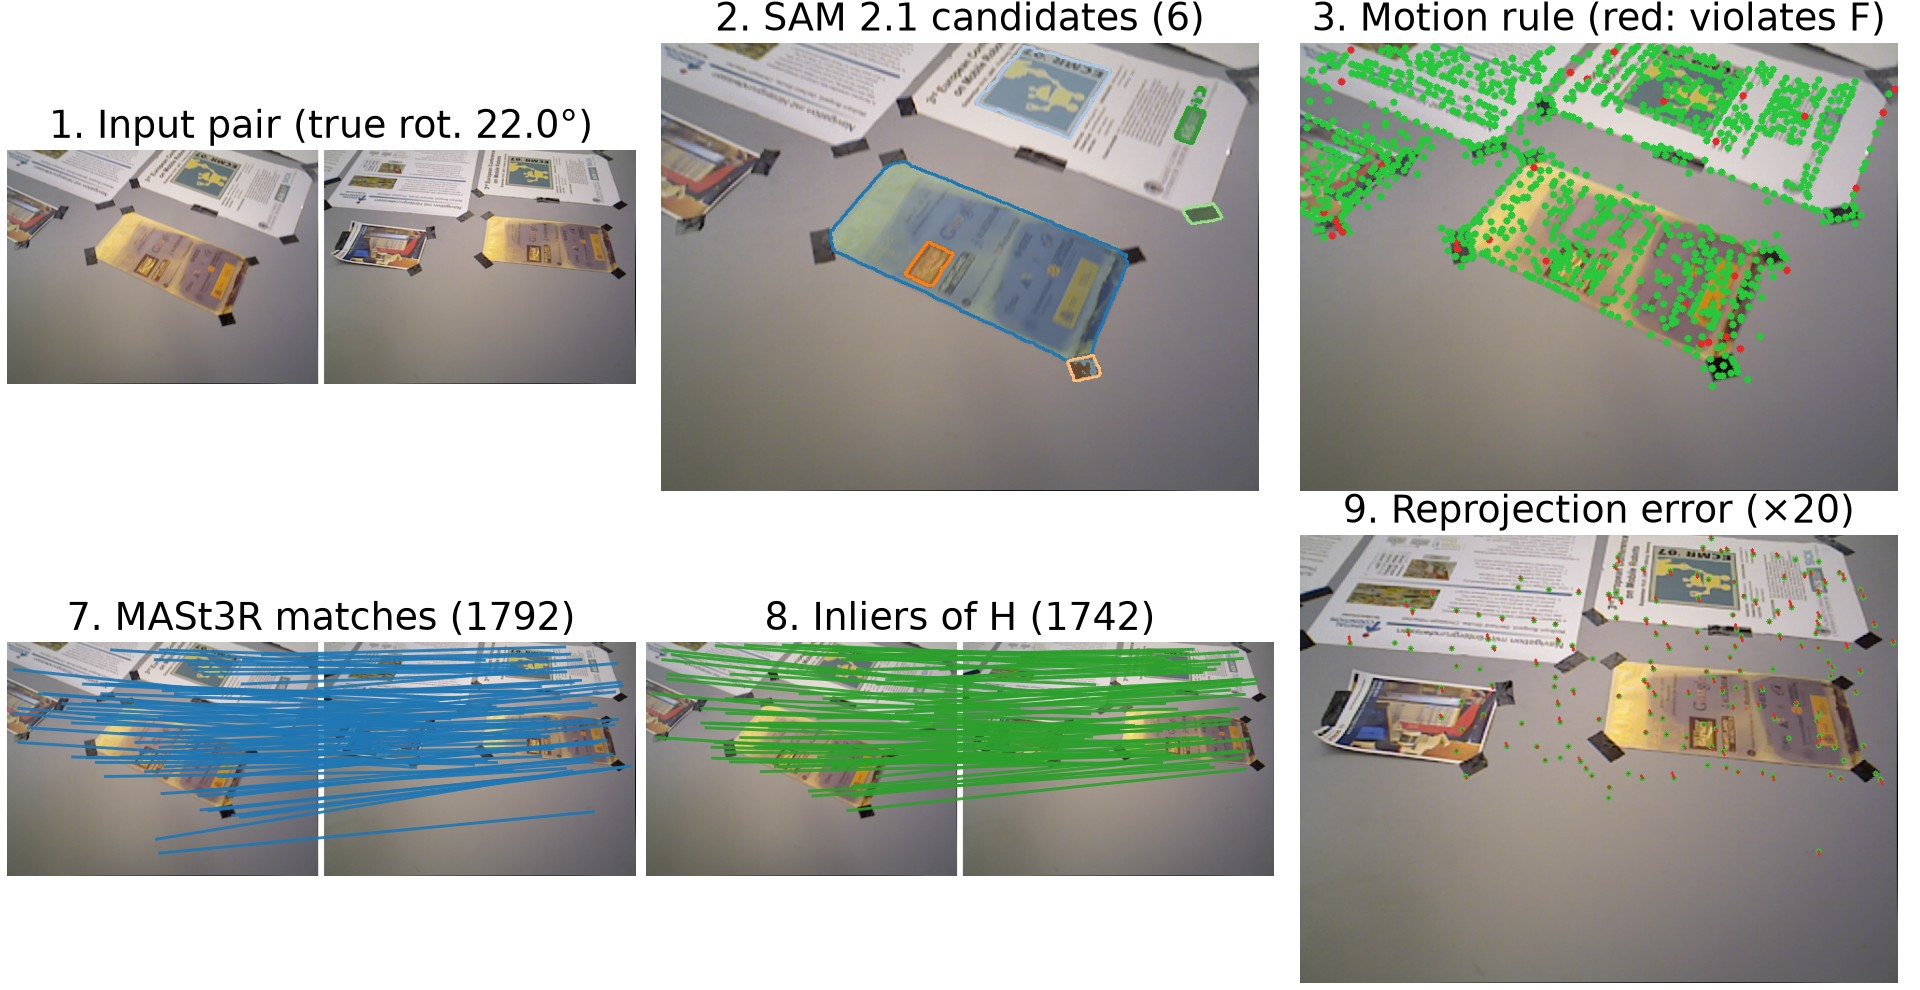
\includegraphics[width=\linewidth]{case_planar_slide.jpg}
    \end{column}
    \begin{column}{0.33\textwidth}
      \small
      \head{TUM poster, true rotation 22.0$^\circ$}
      \begin{enumerate}
        \item SAM 2.1 proposes candidate segments.
        \item All follow the background's motion and align after warping, so the scene is static and the whole images are used.
        \item MASt3R matches; GRIC chooses the model; decomposition and refinement give the pose.
        \item Rotation error \textbf{1.68$^\circ$}, reprojection error \textbf{0.17\,px}.
      \end{enumerate}
      The focal length was estimated; nothing else was given.
    \end{column}
  \end{columns}
\end{frame}

% ------------------------------------------------------------------ 14 euler
\begin{frame}{Results --- roll, pitch and yaw along a sequence}
  \begin{columns}[c]
    \begin{column}{0.42\textwidth}
      \centering
      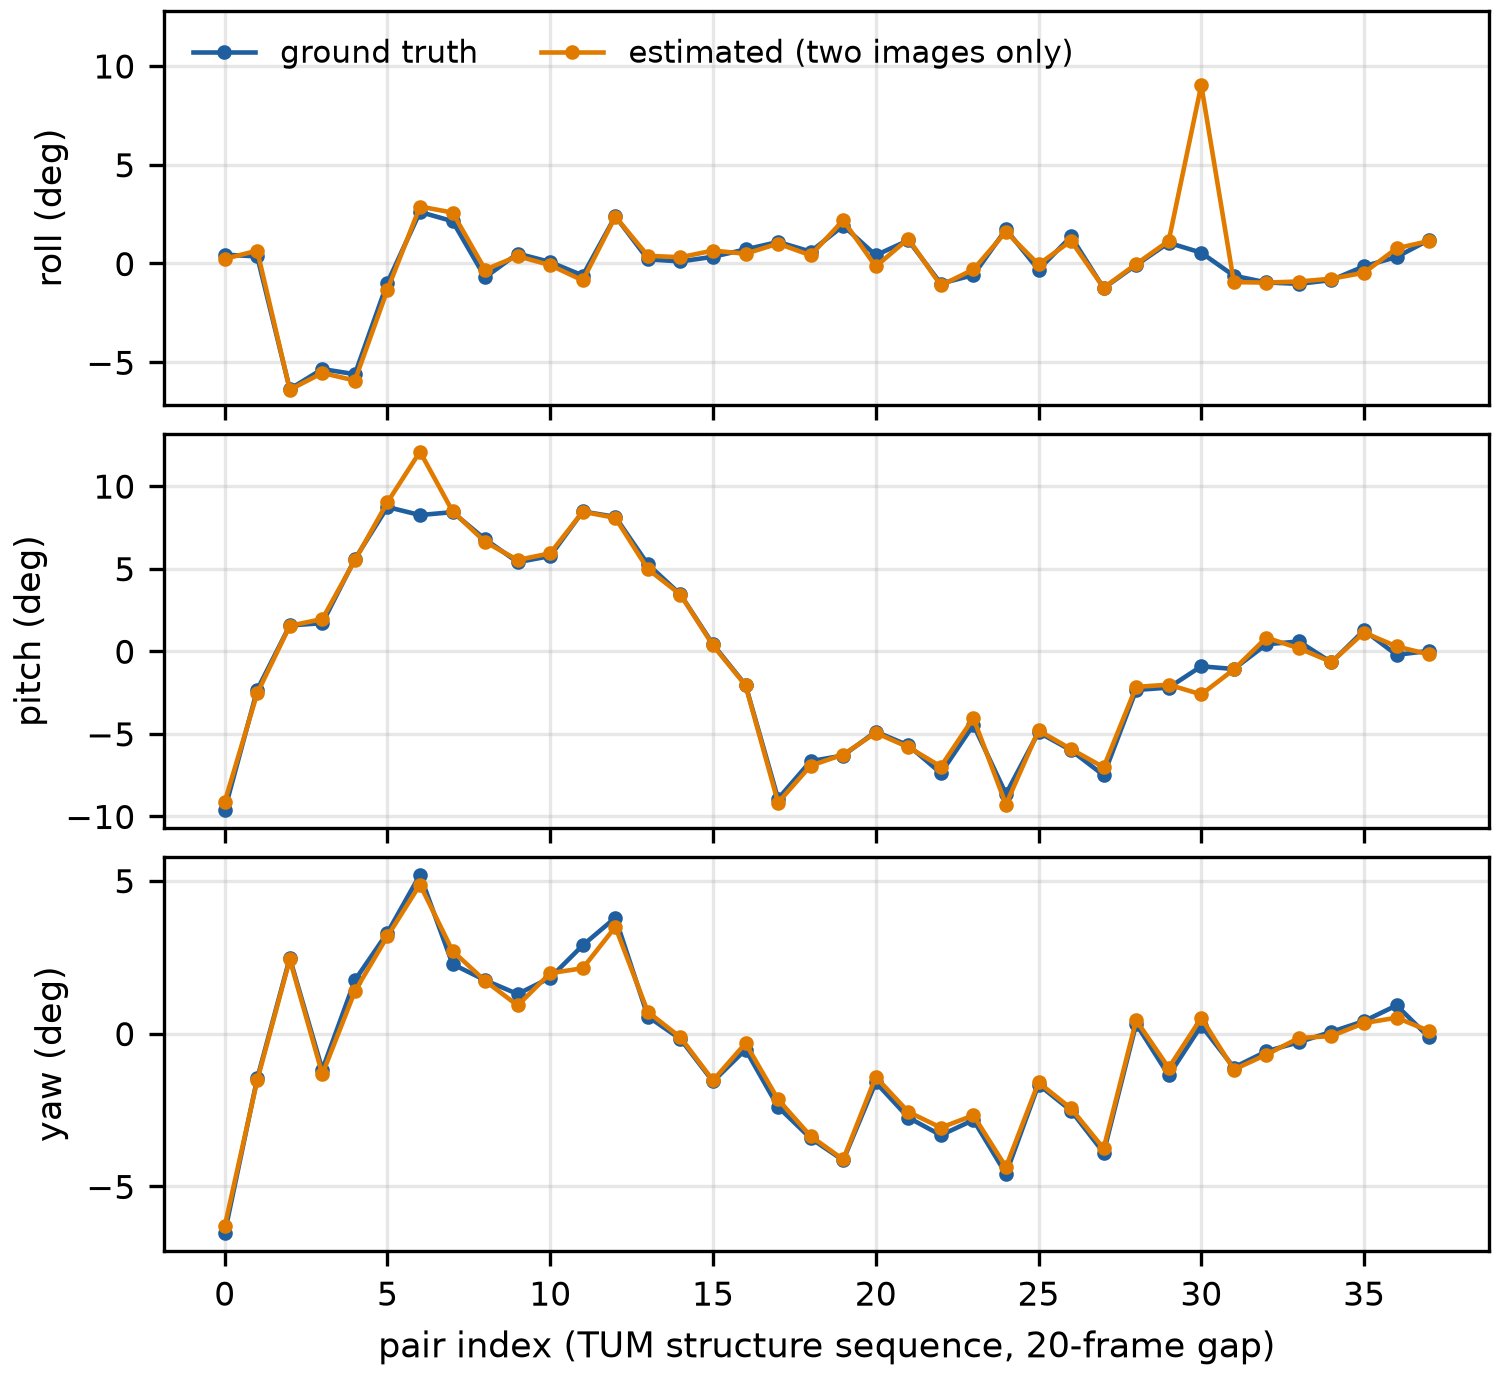
\includegraphics[width=\linewidth]{euler_struct_near_gap20.png}
    \end{column}
    \begin{column}{0.52\textwidth}
      \small
      38 TUM pairs 20 frames apart, each estimated from the two images only. The estimates follow the ground truth closely; the largest deviation is one roll error at pair 30.\\[6pt]
      \centering
      \begin{tabular}{lccc}
        \toprule
        Error & MAE & MAX & STD\\
        \midrule
        Roll & 0.43$^\circ$ & 8.48$^\circ$ & 1.33$^\circ$\\
        Pitch & 0.34$^\circ$ & 3.84$^\circ$ & 0.65$^\circ$\\
        Yaw & 0.19$^\circ$ & 0.75$^\circ$ & 0.14$^\circ$\\
        Translation direction & 8.44$^\circ$ & 57.7$^\circ$ & 11.2$^\circ$\\
        Reprojection & 0.21\,px & 0.33\,px & 0.05\,px\\
        \bottomrule
      \end{tabular}\\[6pt]
      \raggedright On consecutive frames the per-axis rotation MAE is \textbf{0.195$^\circ$}.
    \end{column}
  \end{columns}
\end{frame}

% ------------------------------------------------------------------ 15 methods + failure
\begin{frame}{Results --- where each method wins}
  \begin{columns}[c]
    \begin{column}{0.64\textwidth}
      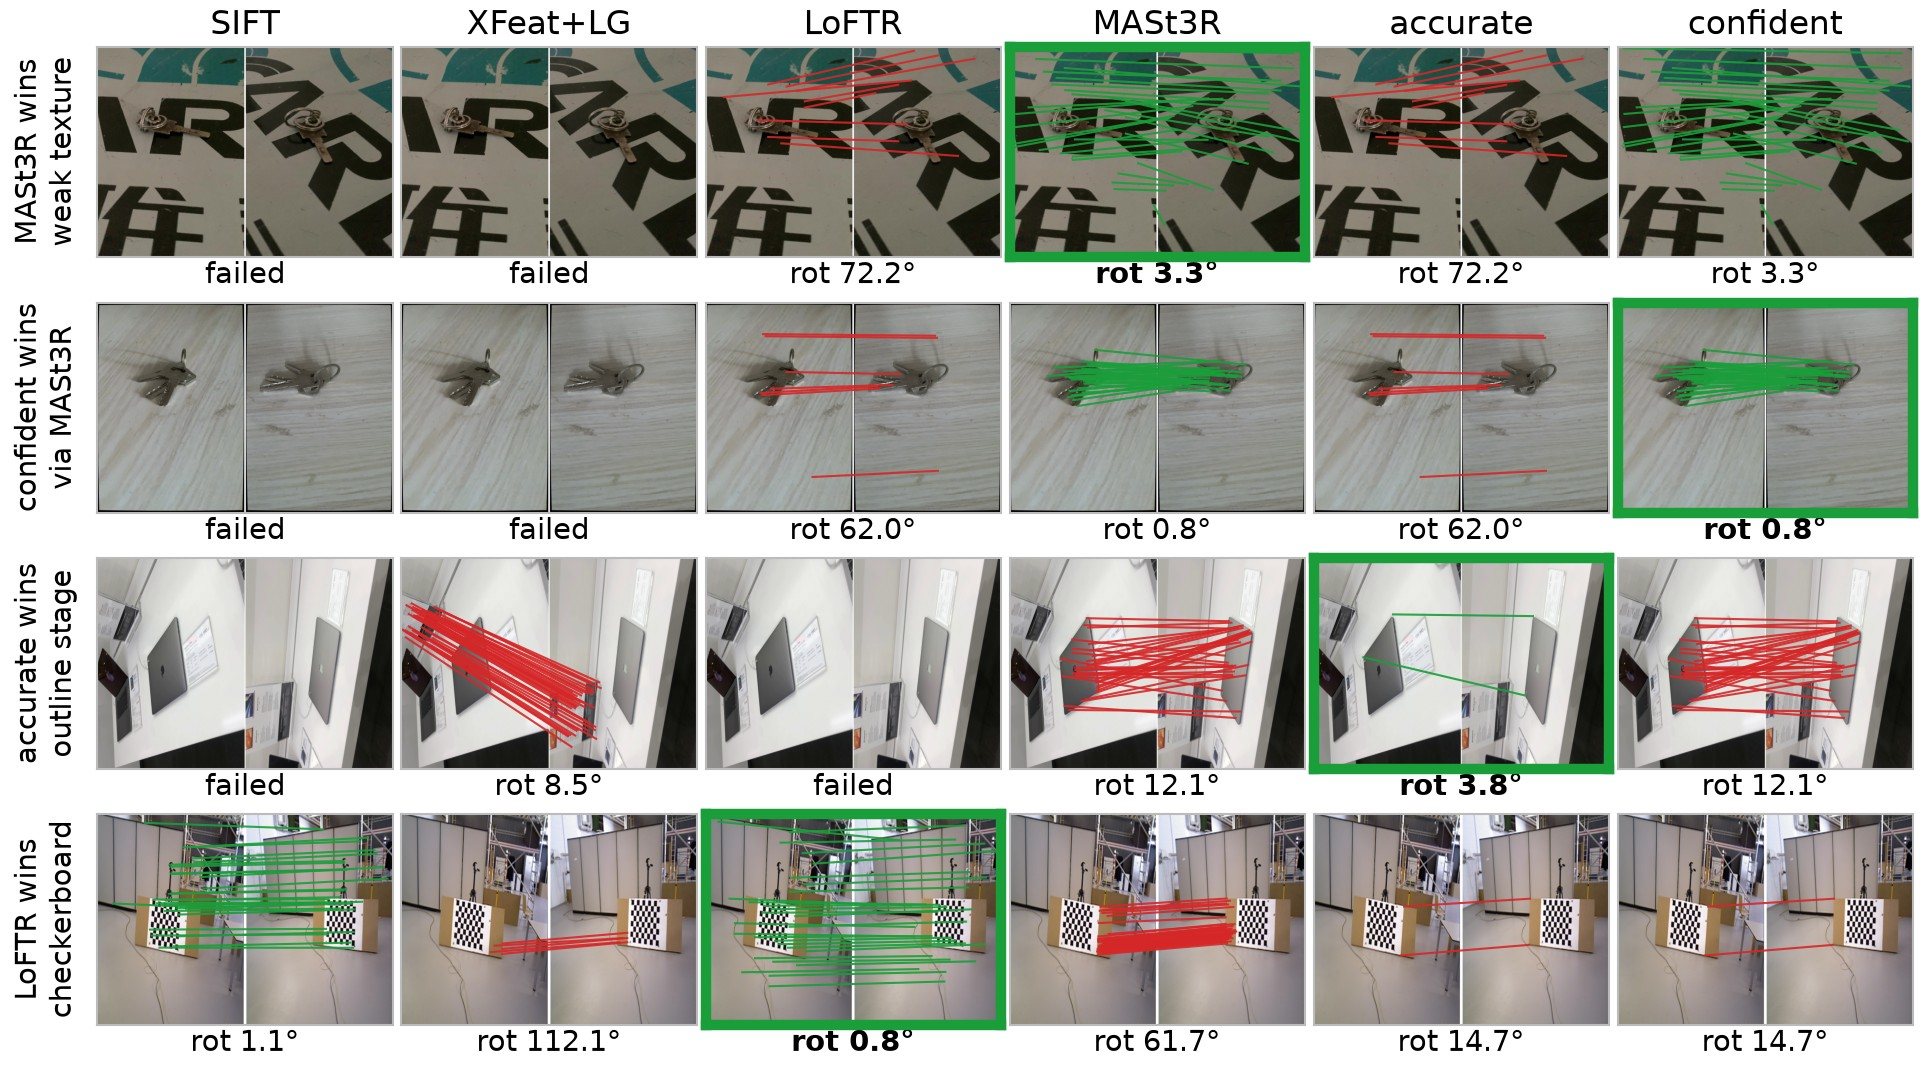
\includegraphics[width=\linewidth]{methods_slide.jpg}
    \end{column}
    \begin{column}{0.33\textwidth}
      \small
      Each row is a pair on which the framed method is clearly best.
      \begin{itemize}
        \item \textbf{MASt3R:} weakly textured keys where the 2D matchers fail.
        \item \textbf{confident:} defers to MASt3R when unsure.
        \item \textbf{accurate:} its outline stage on a laptop.
        \item \textbf{LoFTR:} a checkerboard pair where a wrong region pairing misleads MASt3R ($61.7^\circ$ error at only 0.49\,px).
      \end{itemize}
      \head{Reliability.} When MASt3R and \texttt{accurate} agree within $2^\circ$ (34 of 56 pairs), no rotation error exceeds $10^\circ$.
    \end{column}
  \end{columns}
\end{frame}

% ------------------------------------------------------------------ test sample 1
\begin{frame}{Evaluation on a test sample --- monitor box}
  \begin{columns}[c]
    \begin{column}{0.56\textwidth}
      \centering\scriptsize
      \begin{tabular}{@{}c@{\hspace{3pt}}c@{}}
        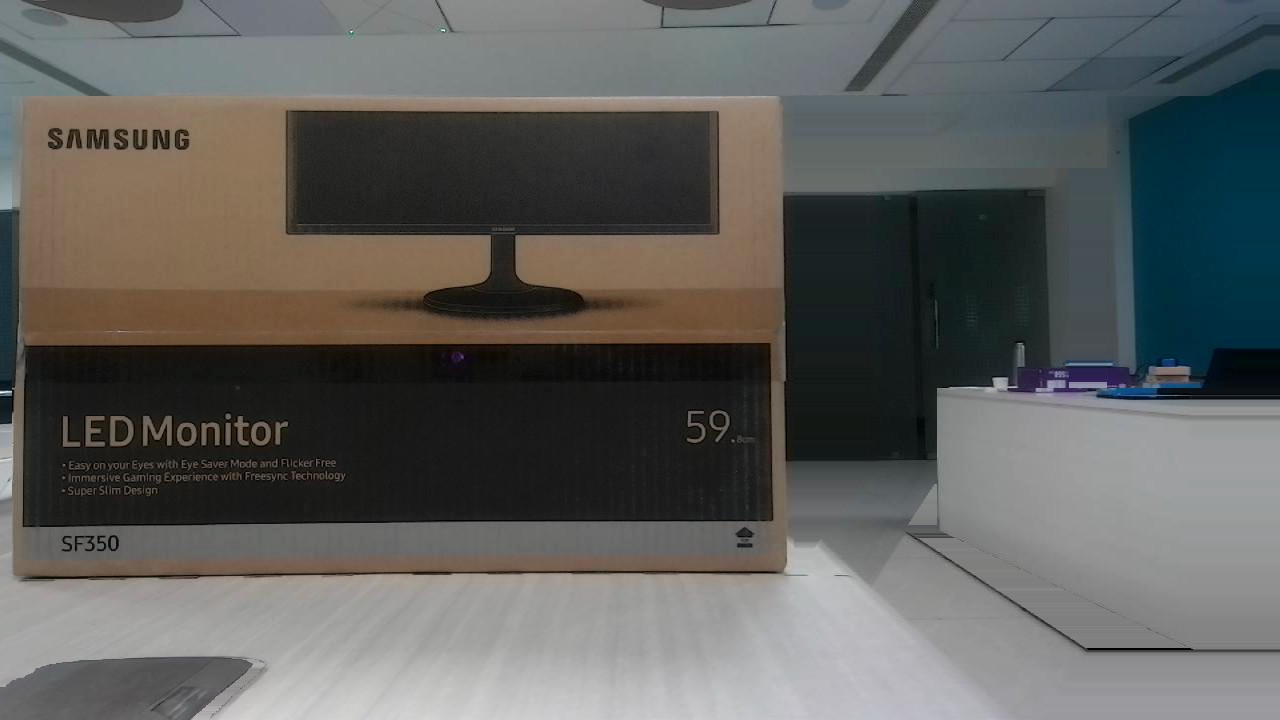
\includegraphics[width=0.4\linewidth]{samples/monitor_box/image1.jpg} &
        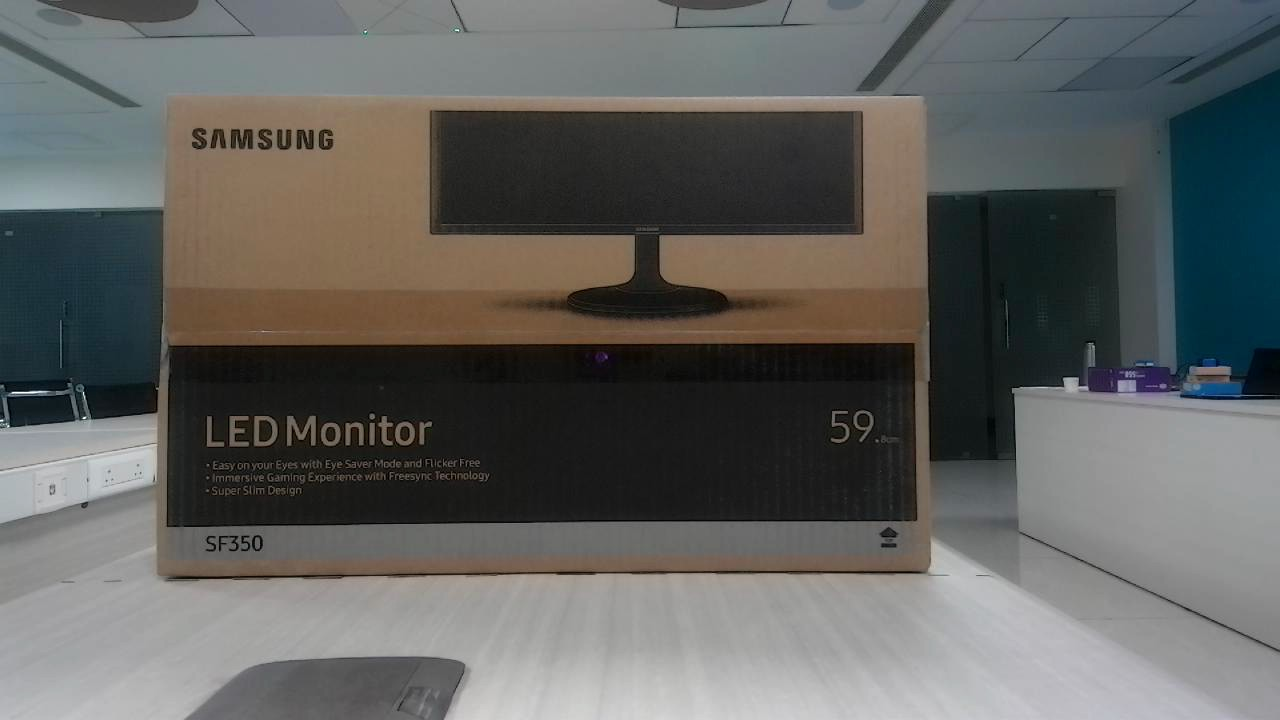
\includegraphics[width=0.4\linewidth]{samples/monitor_box/image2.jpg}\\
        image 1 & image 2\\[2pt]
        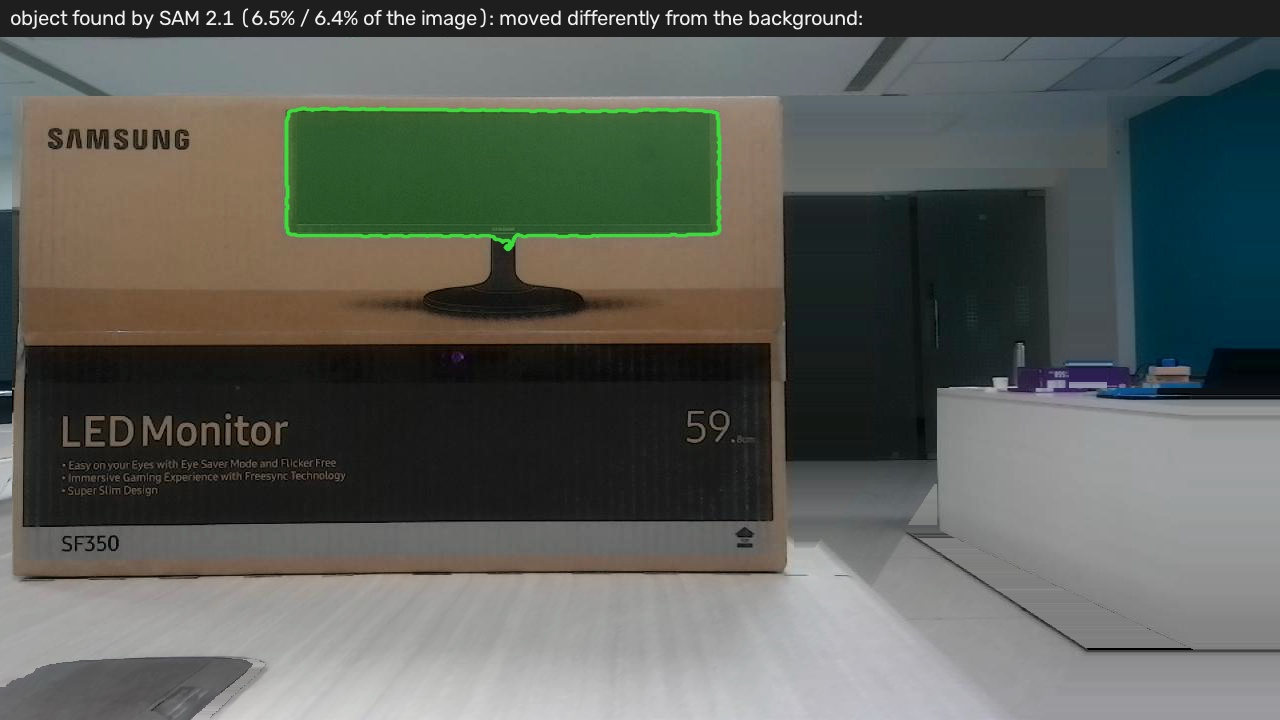
\includegraphics[width=0.4\linewidth]{samples/monitor_box/result_mask1.jpg} &
        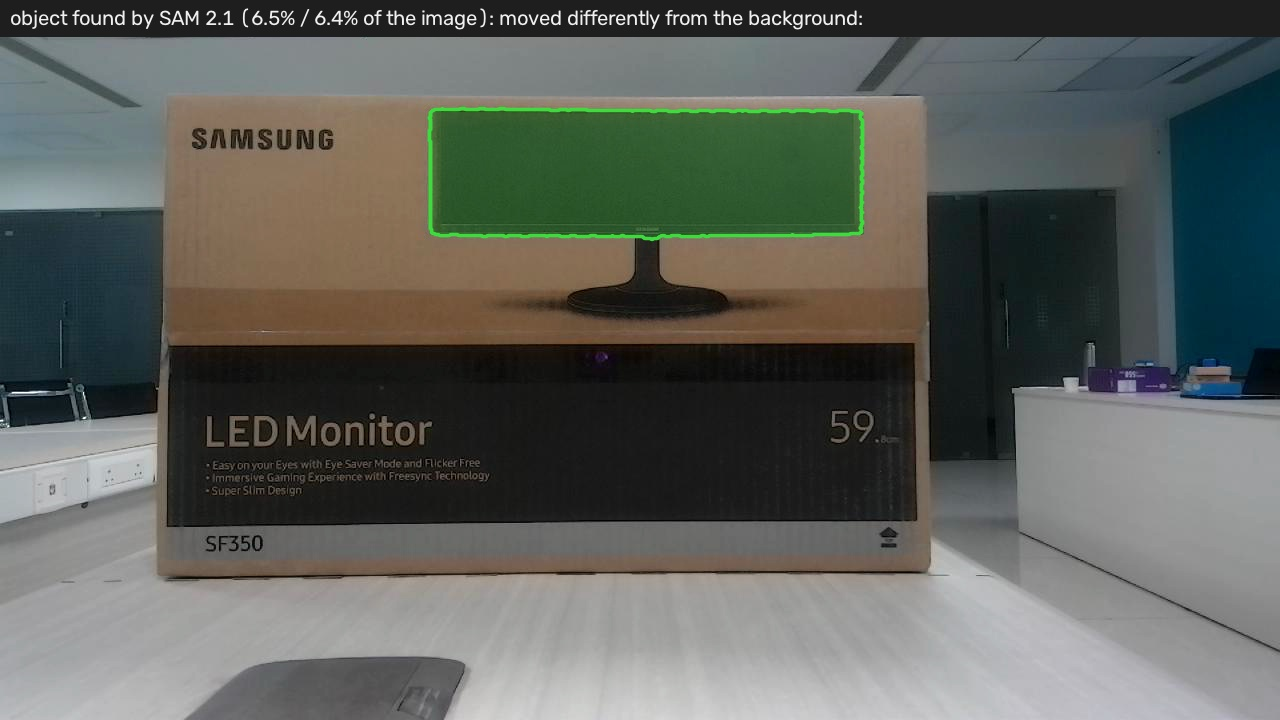
\includegraphics[width=0.4\linewidth]{samples/monitor_box/result_mask2.jpg}\\
        object found (green) & same object in image 2\\[2pt]
        \multicolumn{2}{c}{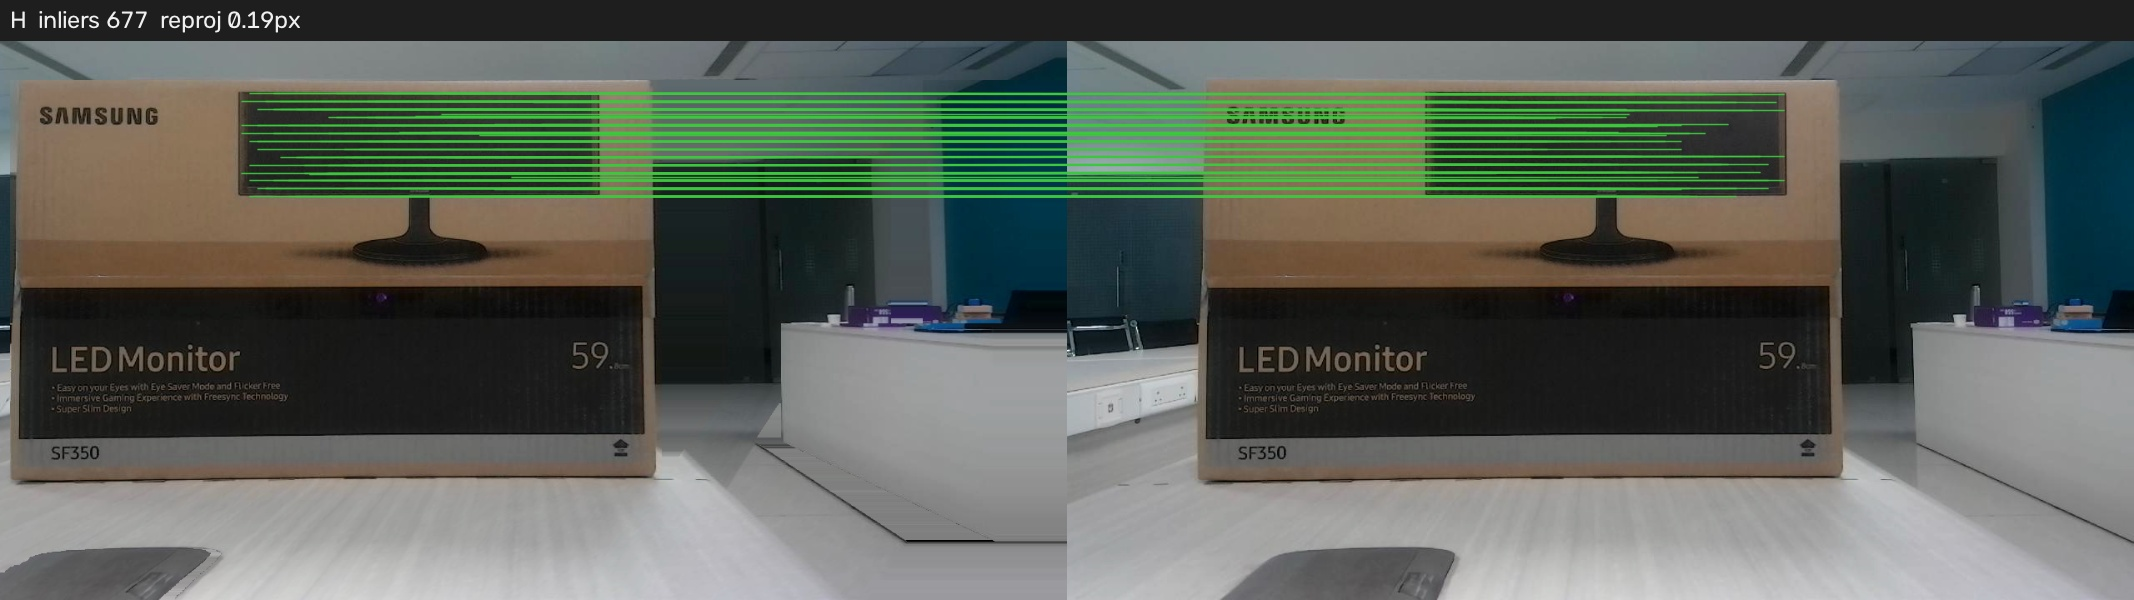
\includegraphics[width=0.82\linewidth]{samples/monitor_box/result.jpg}}\\
        \multicolumn{2}{c}{MASt3R inlier correspondences}
      \end{tabular}
    \end{column}
    \begin{column}{0.42\textwidth}
      \begin{block}{Result (two images only, MASt3R)}
        \scriptsize
        \[\R=\begin{pmatrix}0.99999&-0.00082&-0.00189\\0.00083&0.99998&0.00617\\0.00188&-0.00617&0.99998\end{pmatrix}\]
        \[\tv=(0.998,\,-0.046,\,0.033)\ \text{(direction)}\]
        \begin{tabular}{@{}ll@{}}
          Rotation angle & $0.37^\circ$\\
          Reprojection RMS & 0.19\,px\\
          Model (GRIC) & $H$ (planar)\\
          Inliers / matches & 677 / 677\\
          Focal length & 893\,px (estimated)\\
          Region & moved (motion confirmed)\\
          Pose time & 4.2\,s\\
          Verdict & \textsc{reliable}\\
        \end{tabular}
      \end{block}
      \footnotesize The box slid sideways without turning: almost no rotation, and the translation points along the camera's $x$ axis.
    \end{column}
  \end{columns}
\end{frame}

% ------------------------------------------------------------------ test sample 2
\begin{frame}{Evaluation on a test sample --- alloy wheel}
  \begin{columns}[c]
    \begin{column}{0.56\textwidth}
      \centering\scriptsize
      \begin{tabular}{@{}c@{\hspace{3pt}}c@{}}
        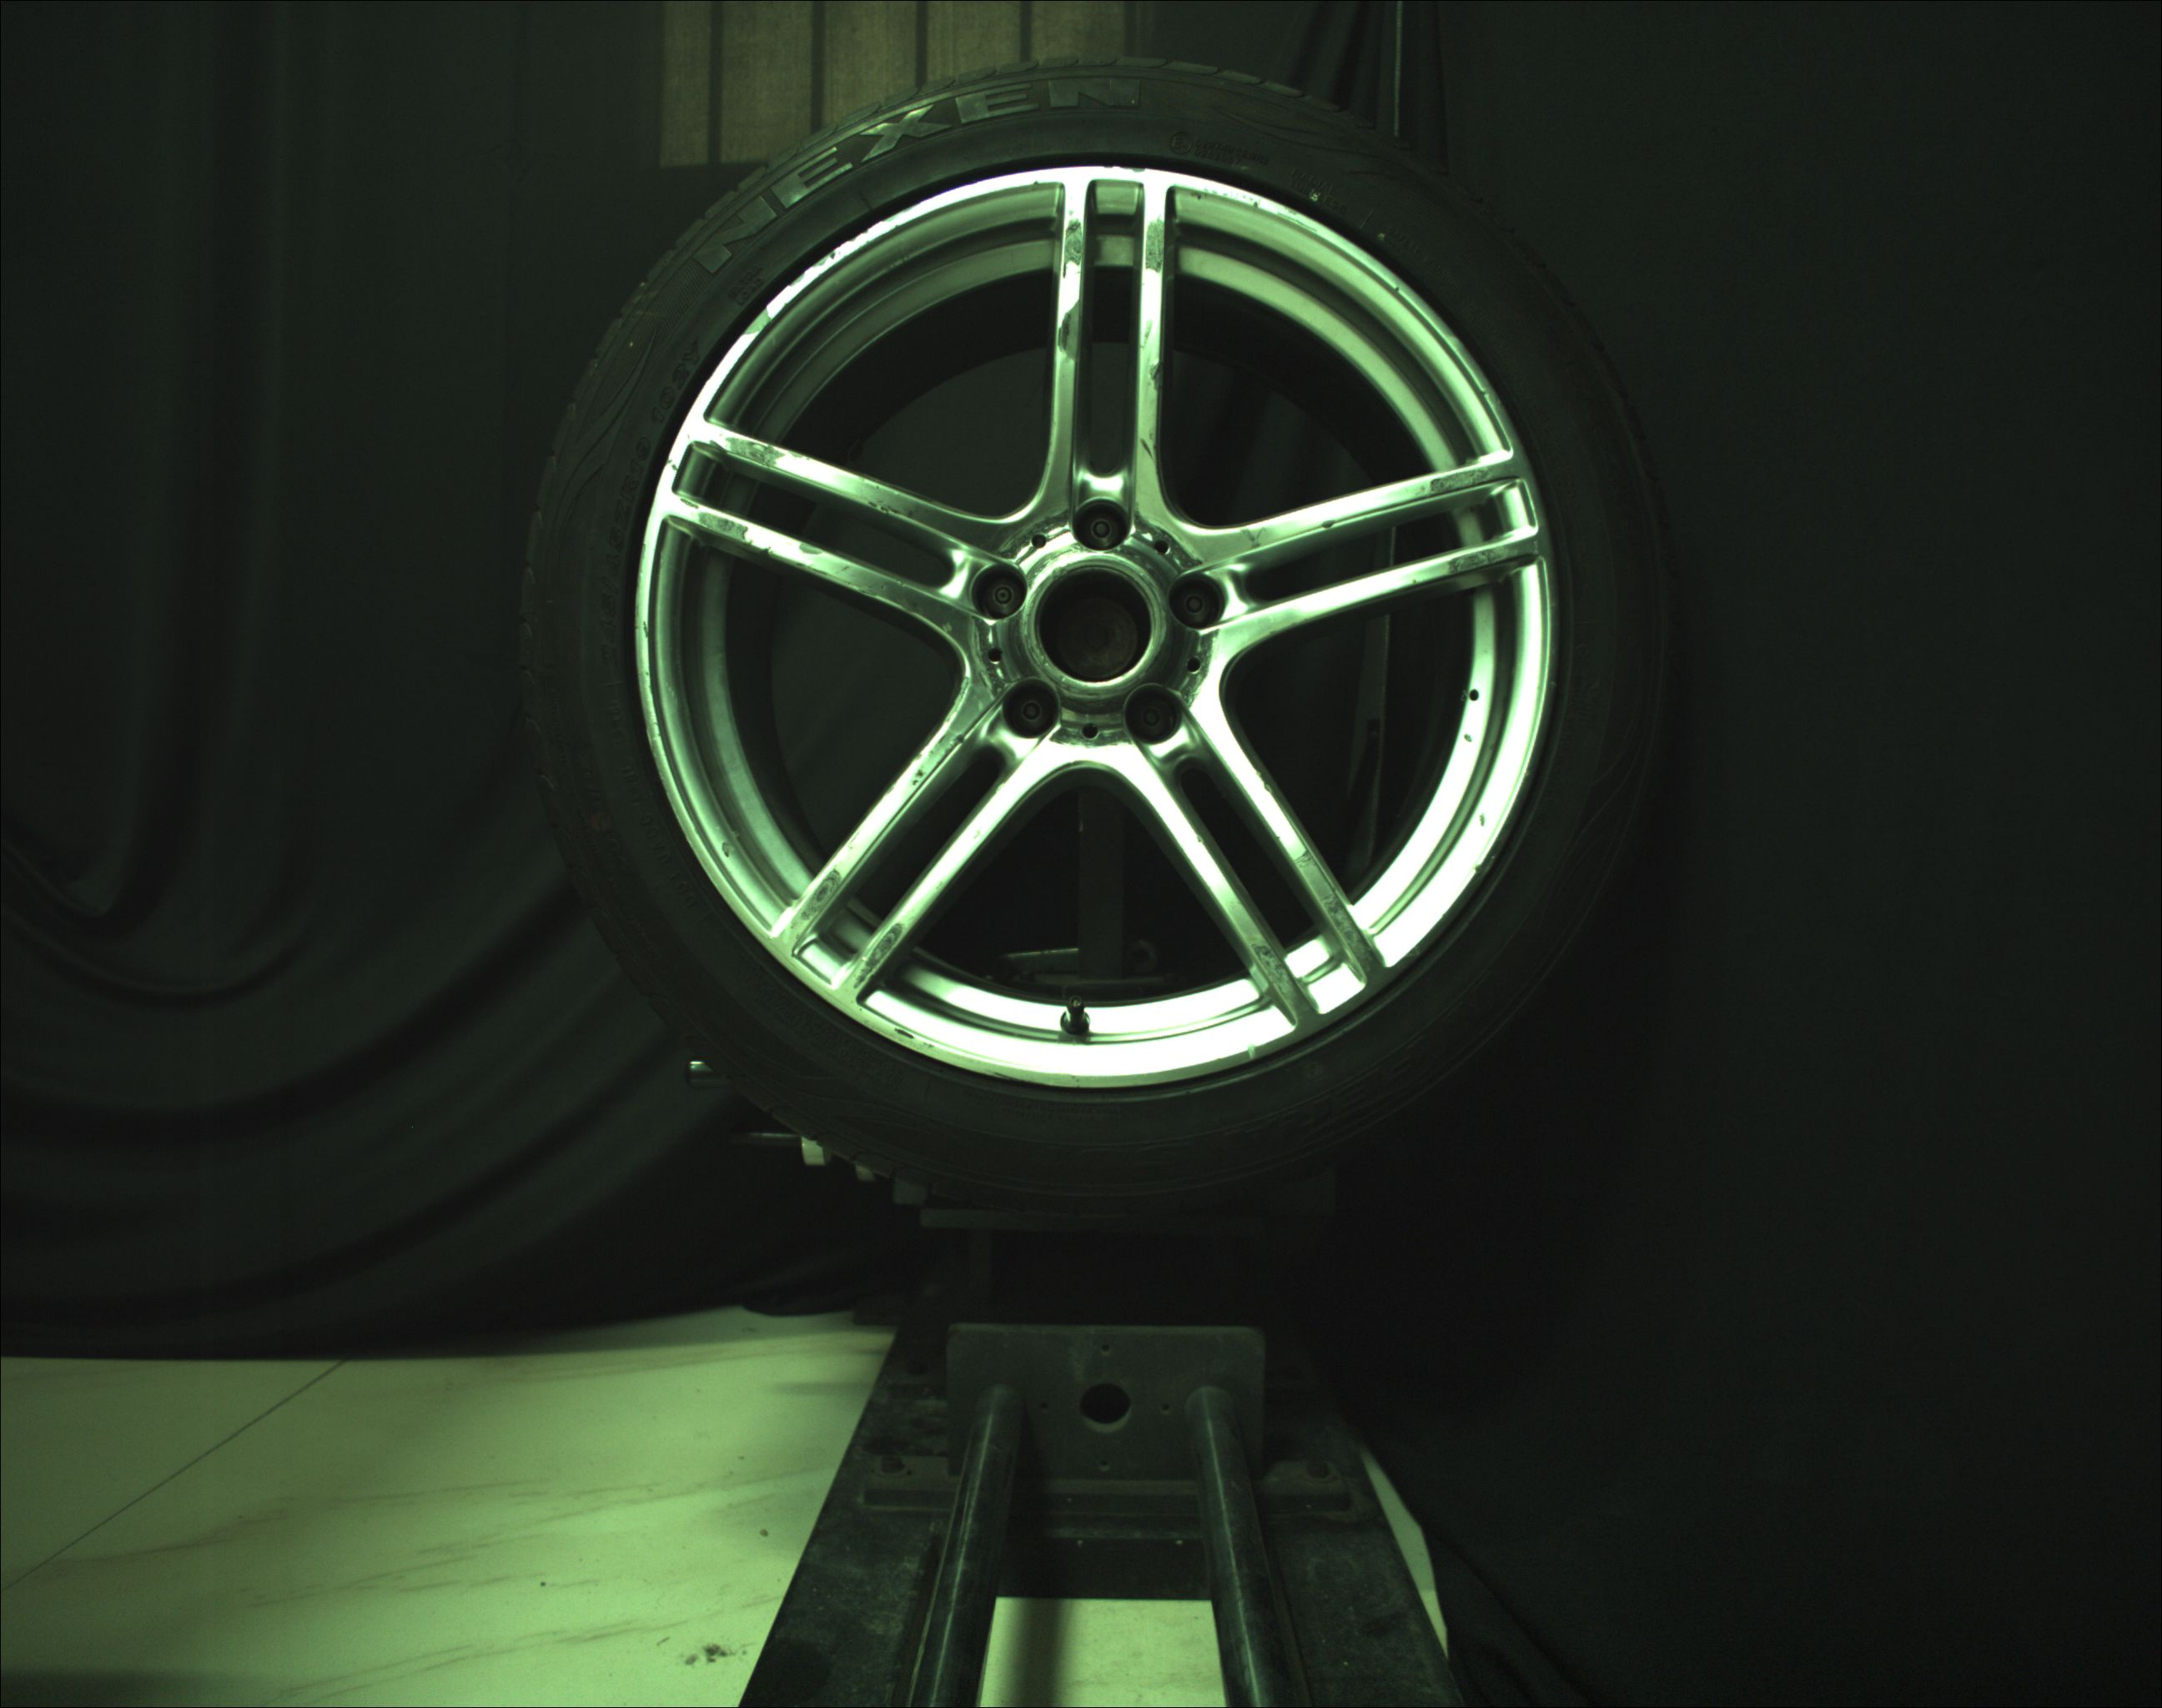
\includegraphics[width=0.29\linewidth]{samples/sample_12/image1.jpg} &
        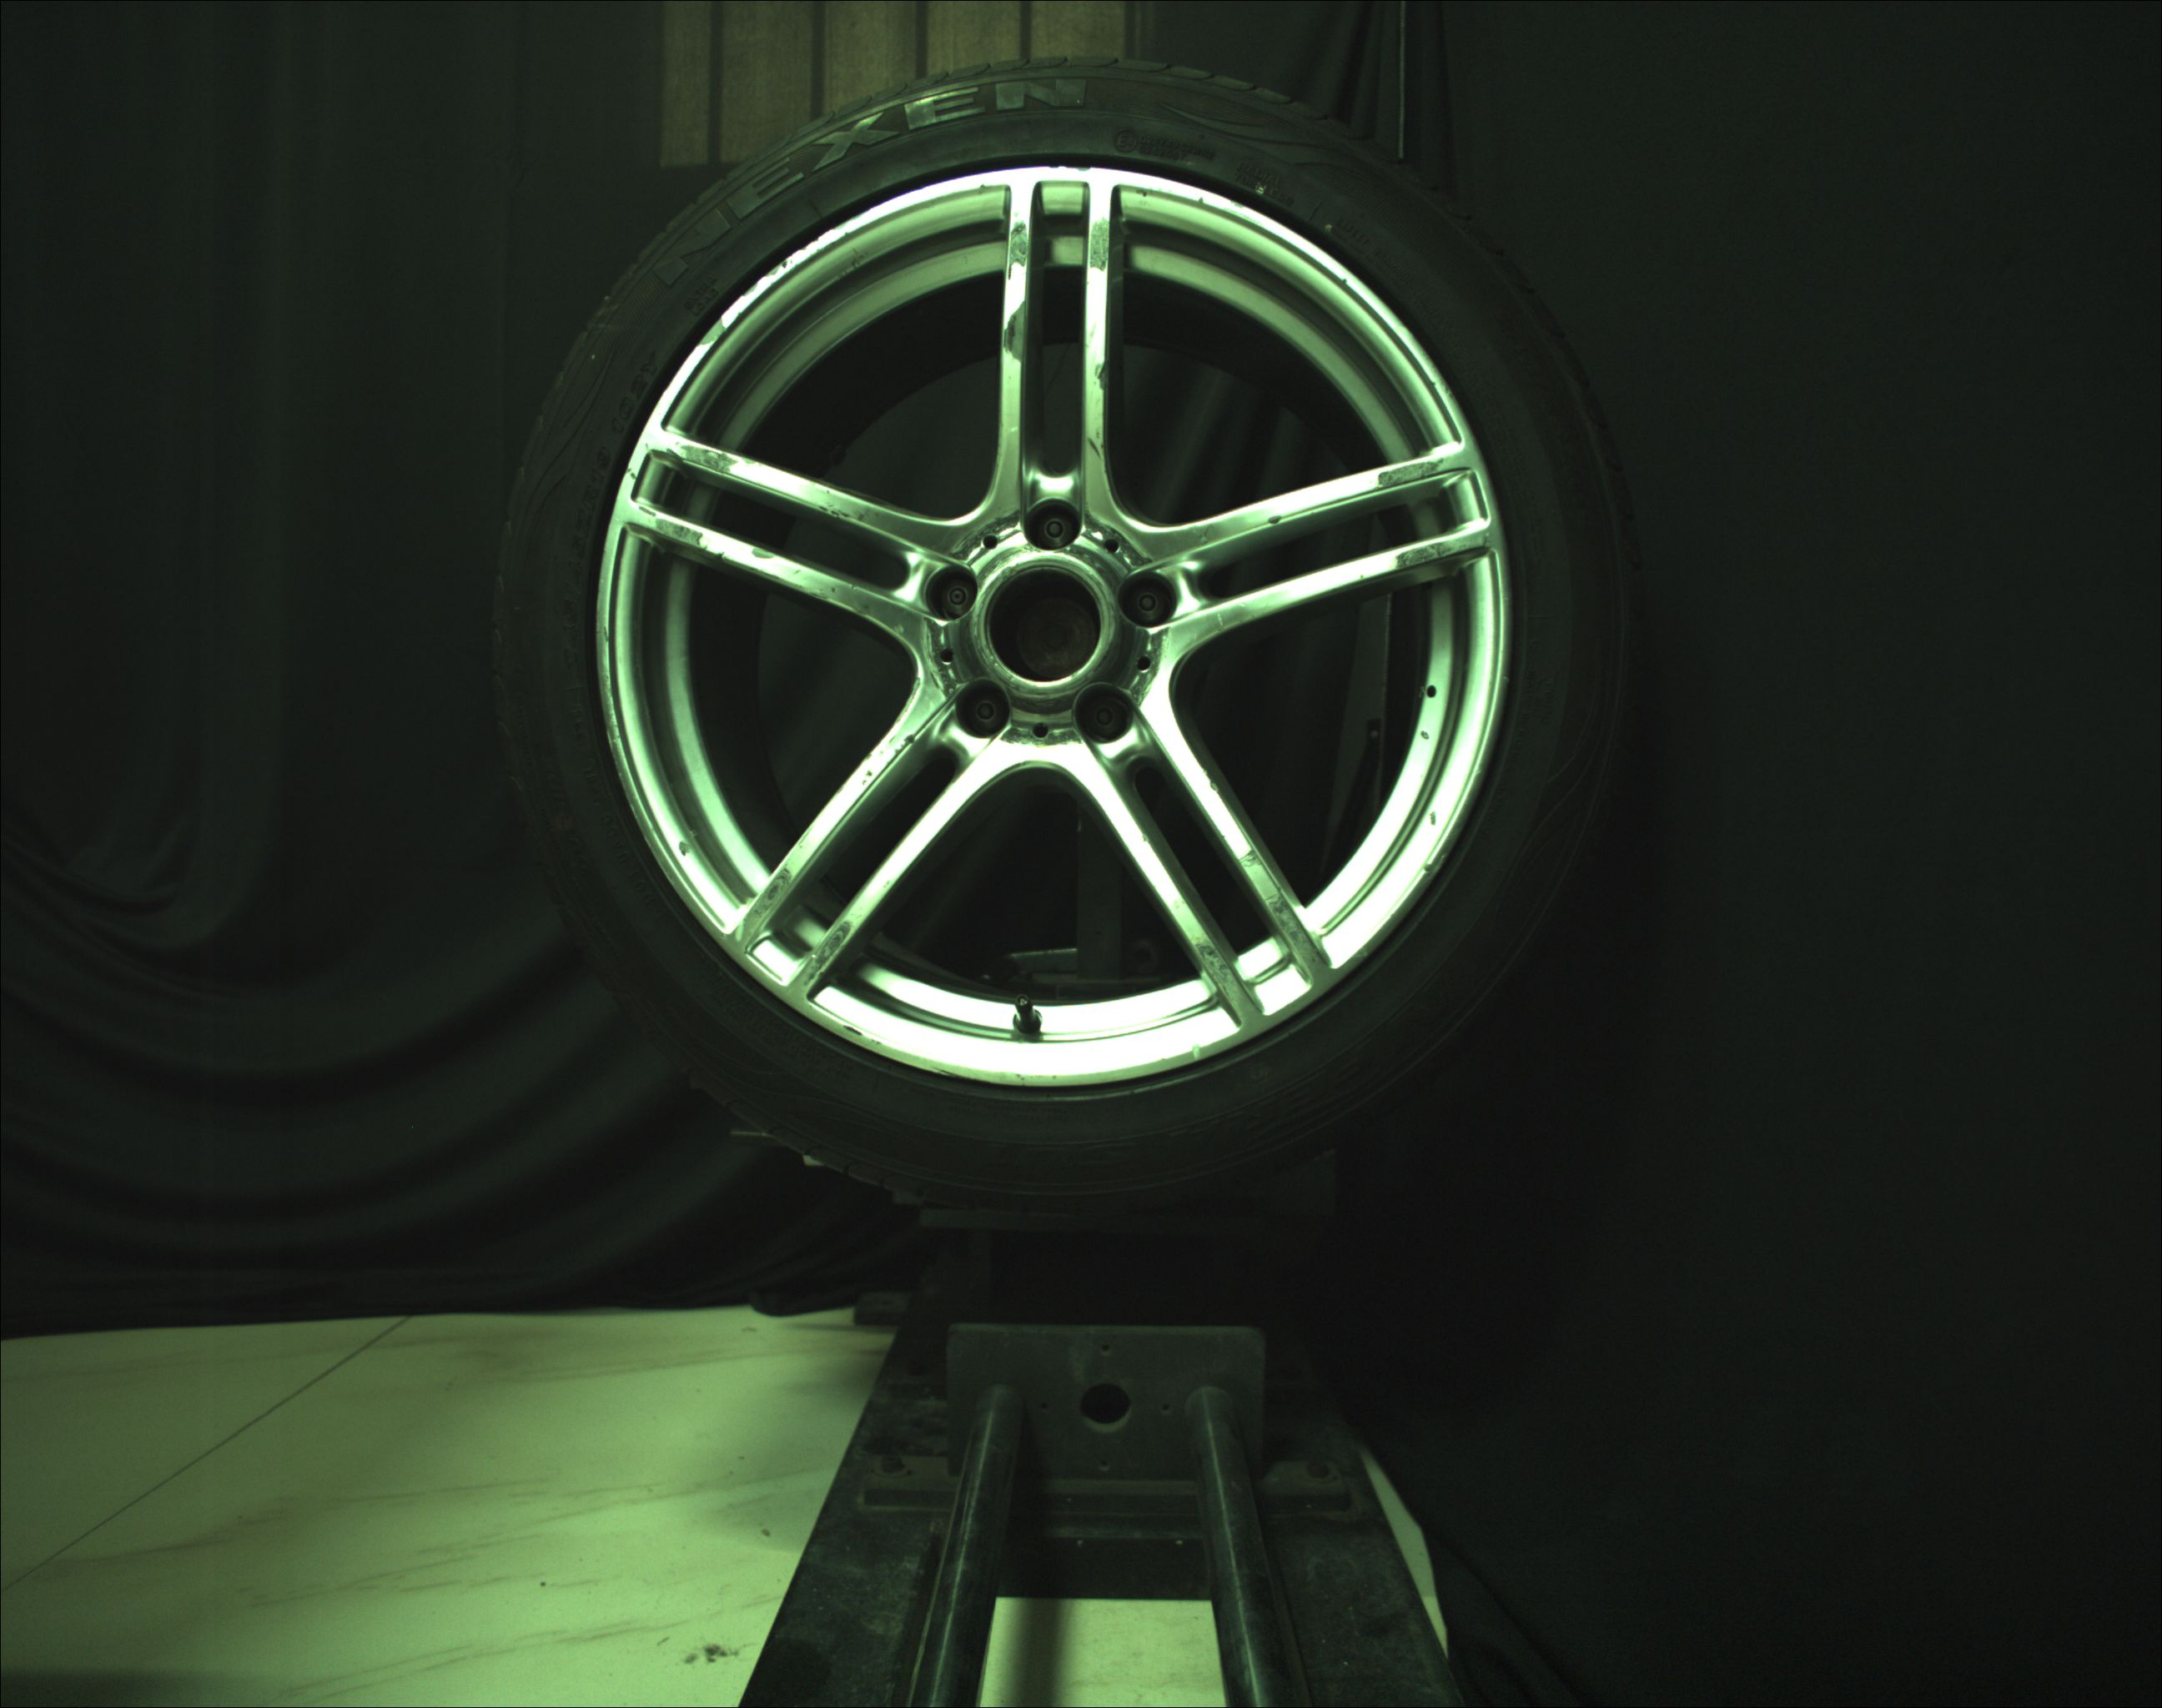
\includegraphics[width=0.29\linewidth]{samples/sample_12/image2.jpg}\\
        image 1 & image 2\\[2pt]
        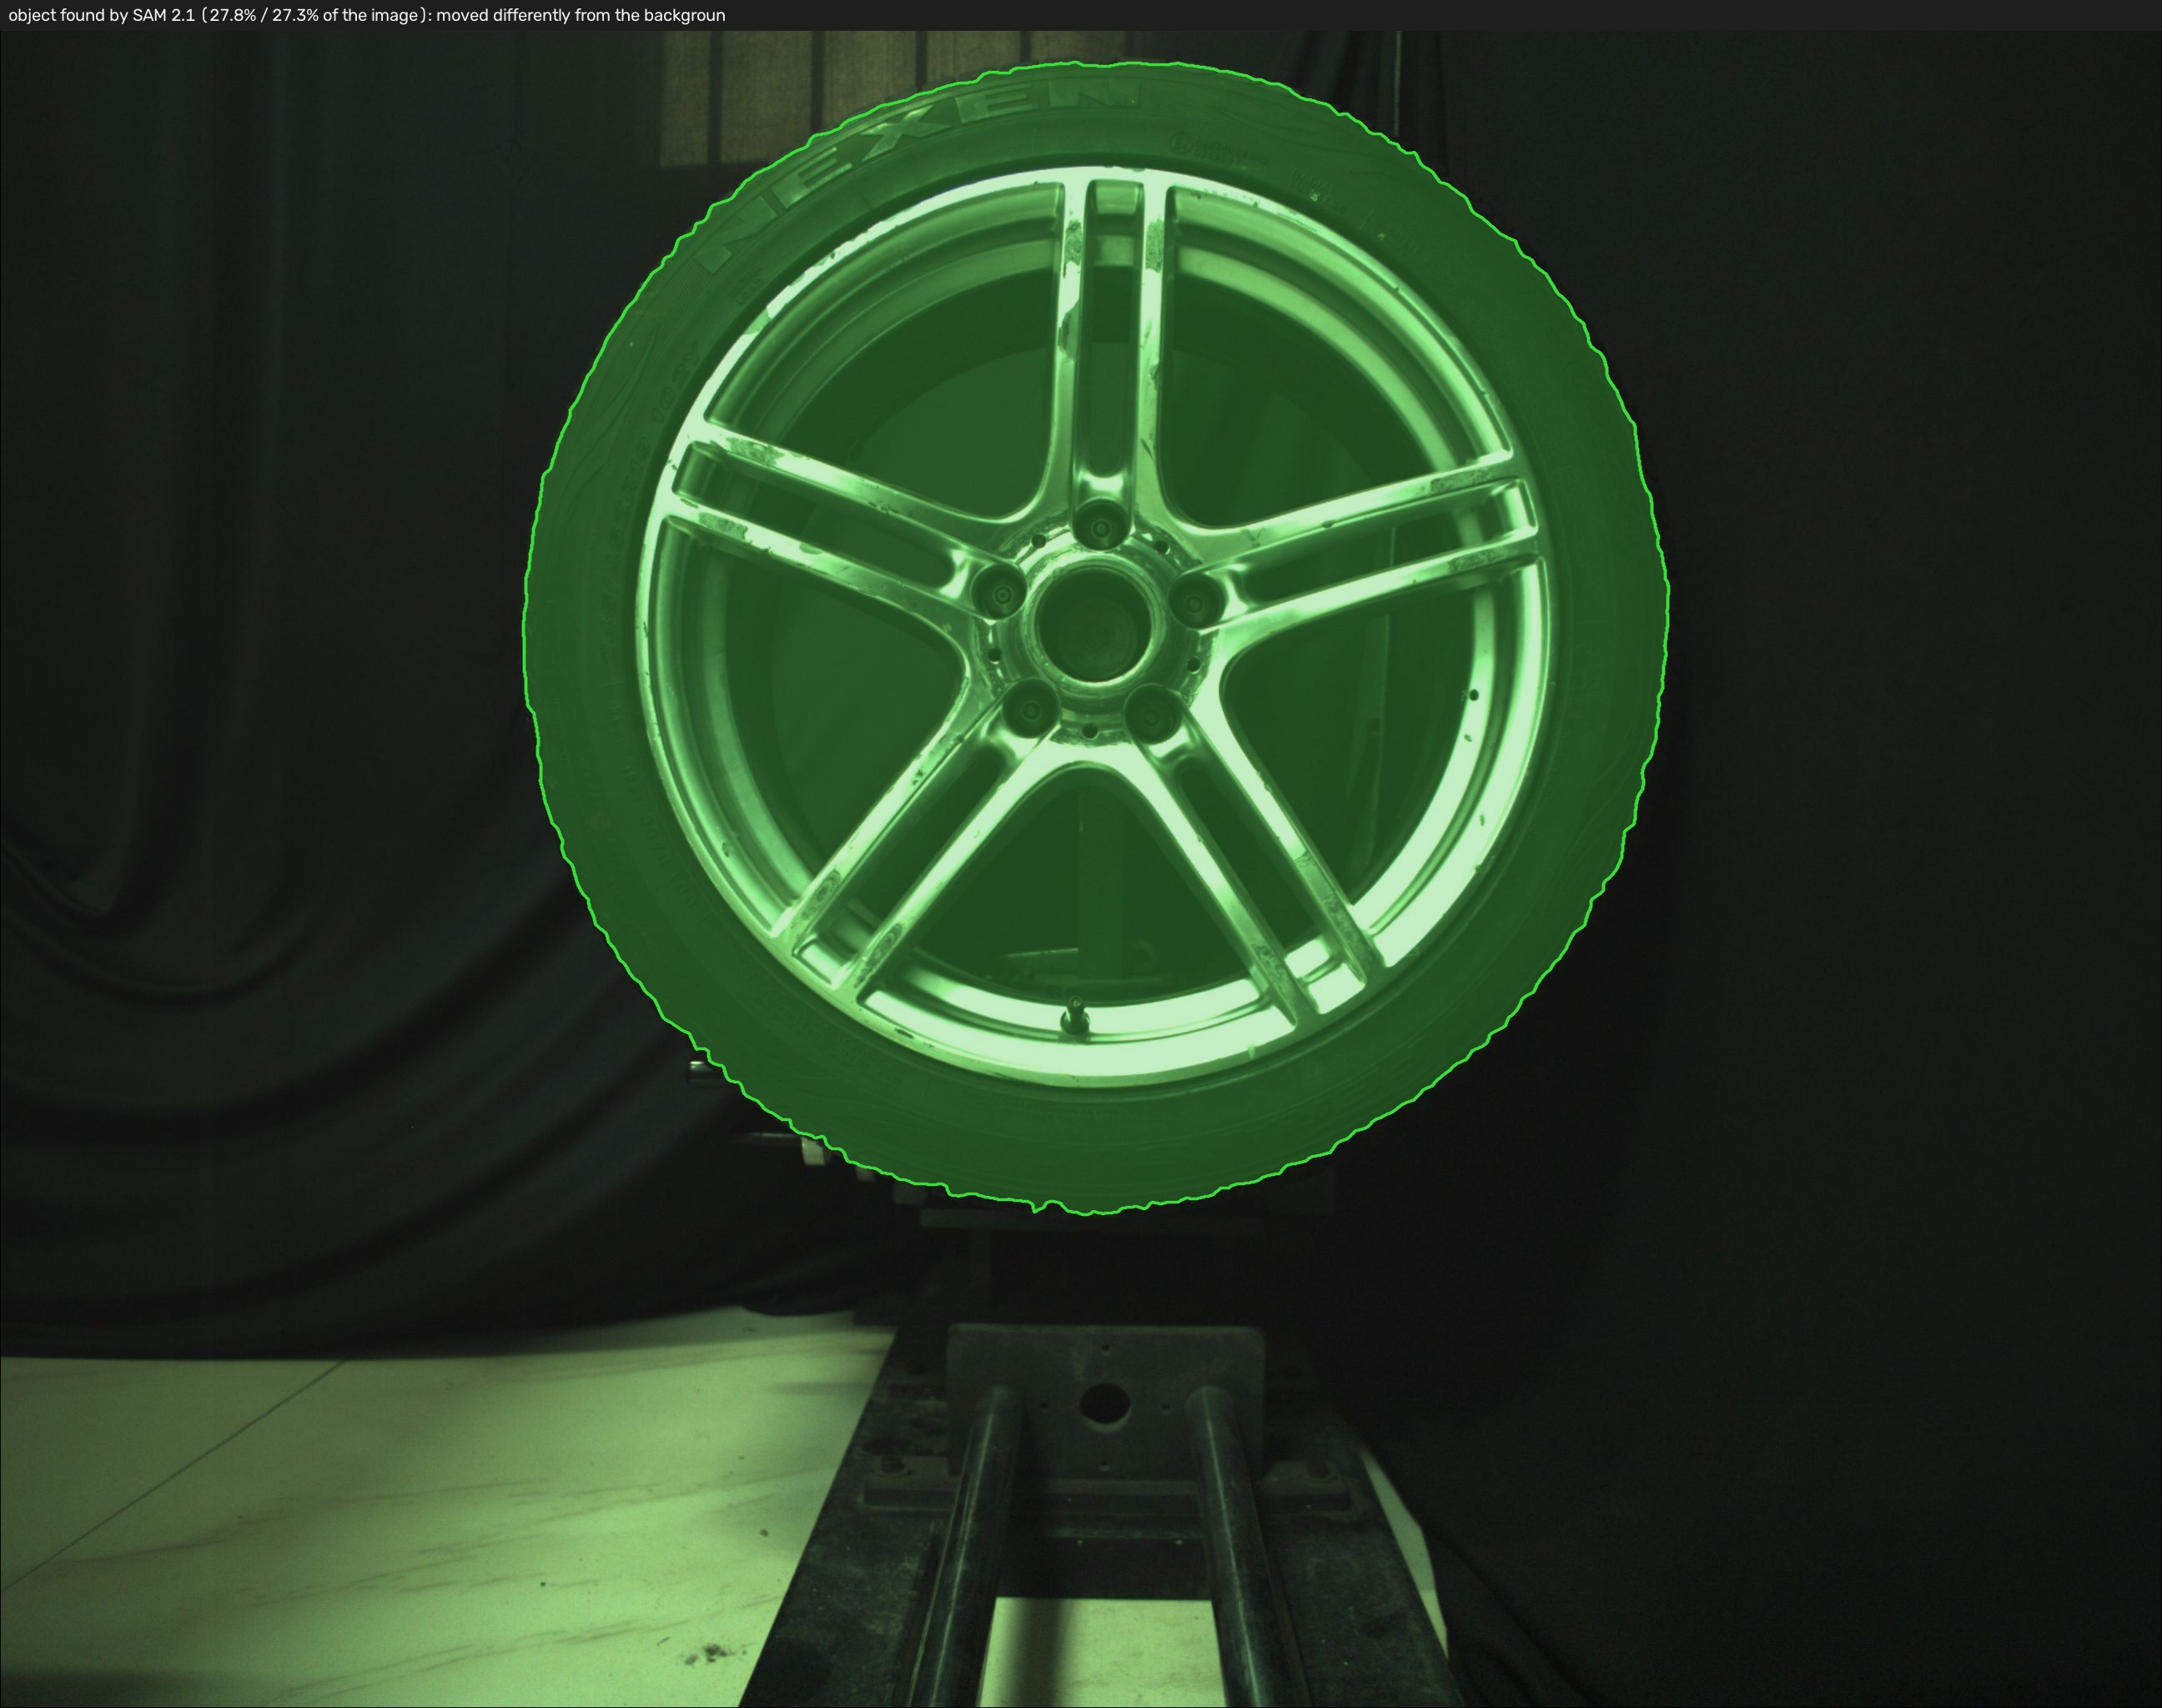
\includegraphics[width=0.29\linewidth]{samples/sample_12/result_mask1.jpg} &
        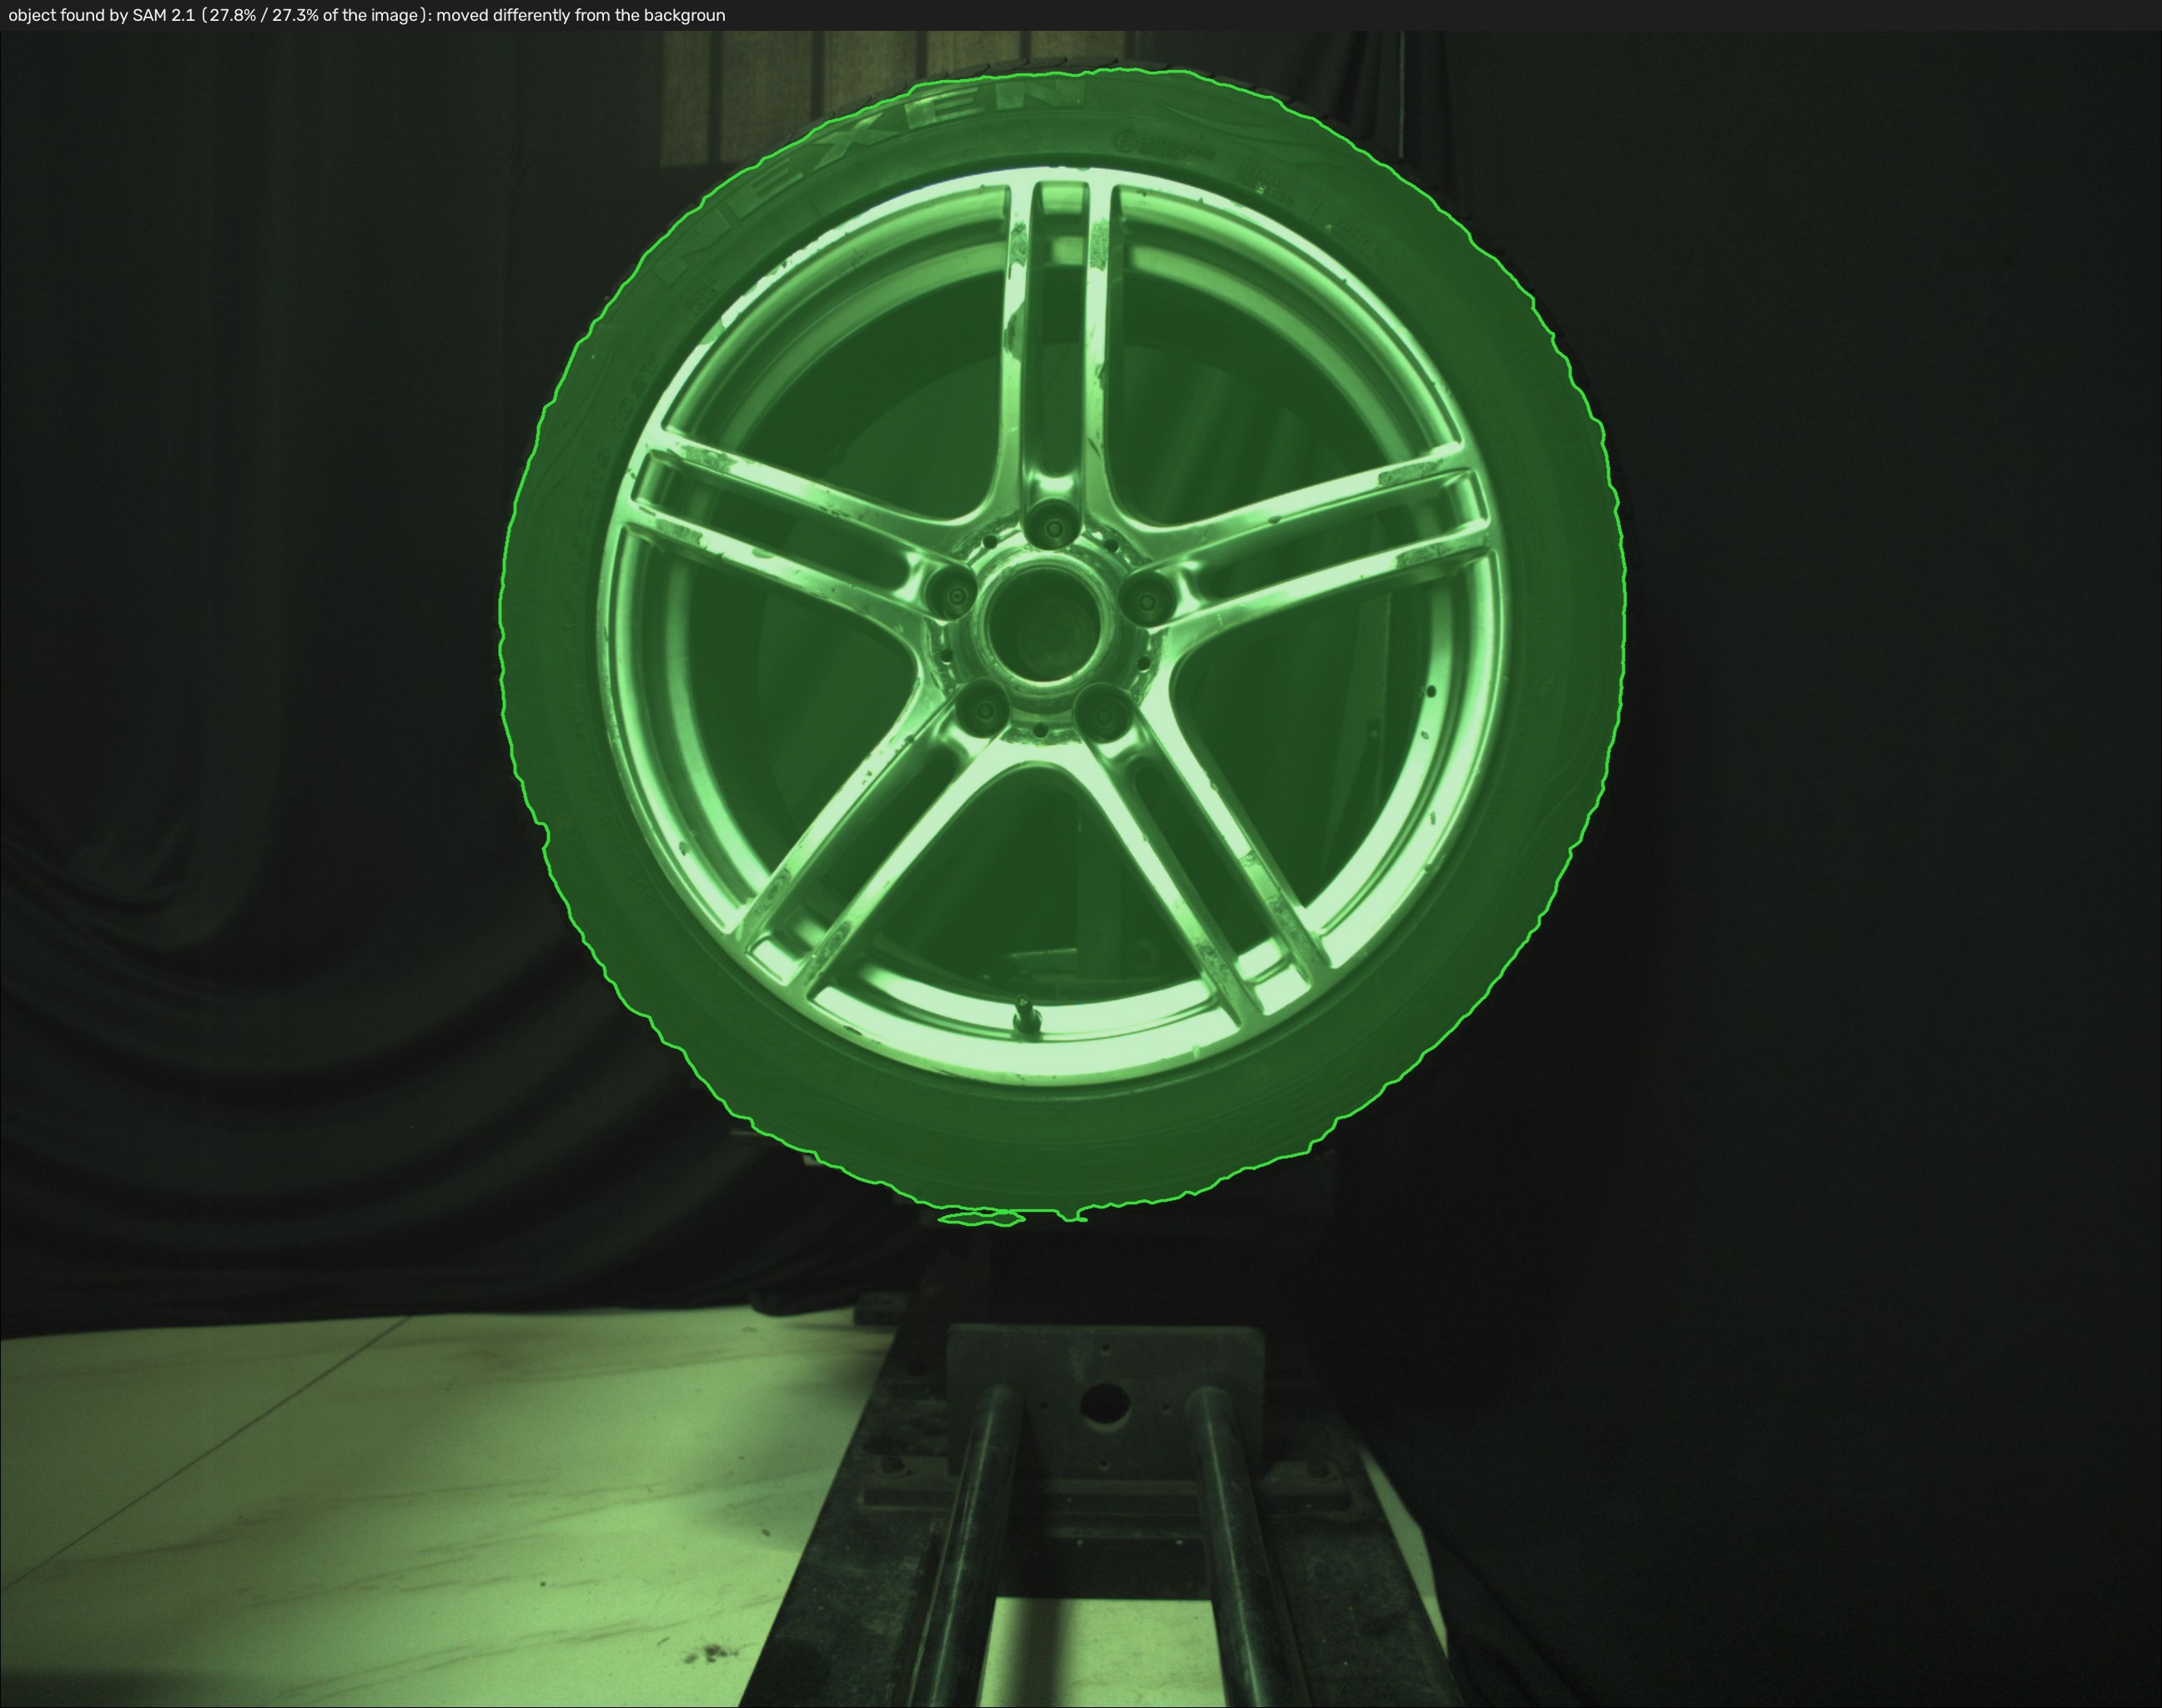
\includegraphics[width=0.29\linewidth]{samples/sample_12/result_mask2.jpg}\\
        object found (green) & same object in image 2\\[2pt]
        \multicolumn{2}{c}{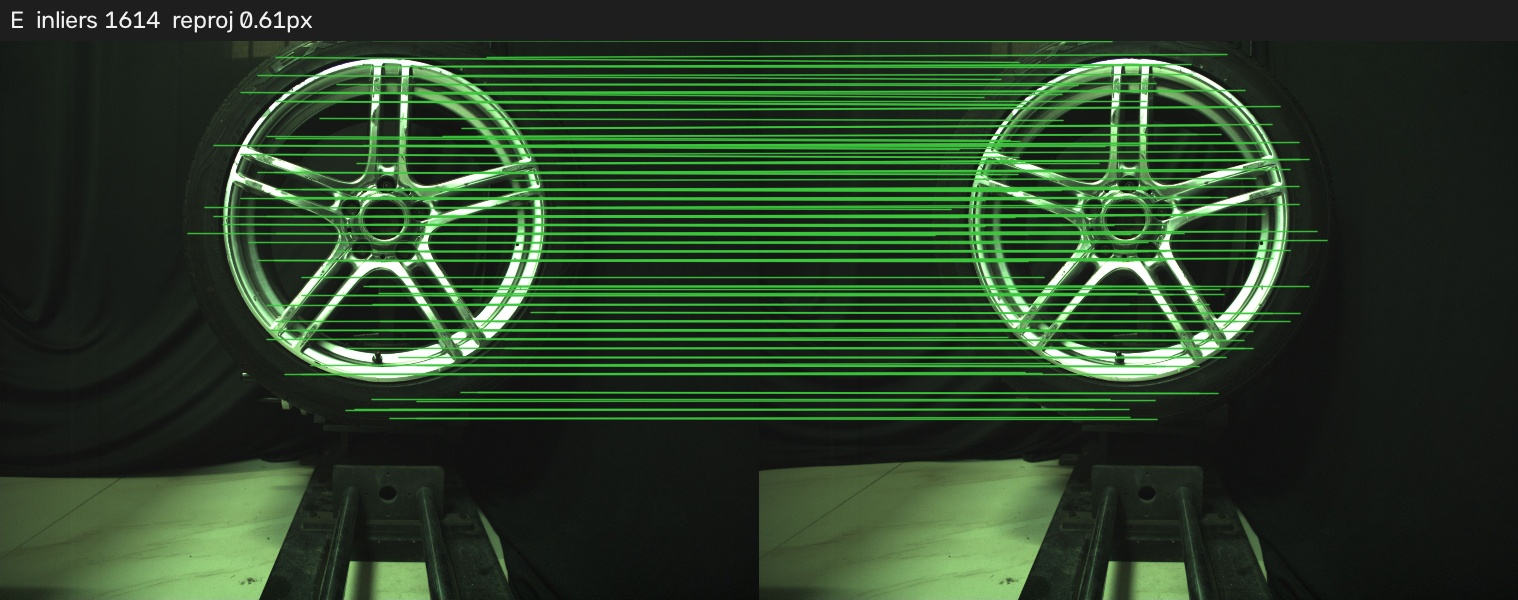
\includegraphics[width=0.6\linewidth]{samples/sample_12/result.jpg}}\\
        \multicolumn{2}{c}{MASt3R inlier correspondences}
      \end{tabular}
    \end{column}
    \begin{column}{0.42\textwidth}
      \begin{block}{Result (two images only, MASt3R)}
        \scriptsize
        \[\R=\begin{pmatrix}0.99789&-0.00054&0.06493\\0.00057&1.00000&-0.00037\\-0.06493&0.00040&0.99789\end{pmatrix}\]
        \[\tv=(-0.999,\,-0.001,\,0.050)\ \text{(direction)}\]
        \begin{tabular}{@{}ll@{}}
          Rotation angle & $3.72^\circ$\\
          Rotation axis & $\approx(0.01,\,1.00,\,0.01)$, vertical\\
          Reprojection RMS & 0.61\,px\\
          Model (GRIC) & $E$ (3D)\\
          Inliers / matches & 1614 / 1614\\
          Focal length & 1498\,px (estimated)\\
          Region & moved (motion confirmed)\\
          Pose time & 18.8\,s\\
          Verdict & \textsc{reliable}\\
        \end{tabular}
      \end{block}
      \footnotesize The wheel turned by about $3.7^\circ$ about the vertical axis and shifted along $-x$; the whole wheel with its tyre was segmented.
    \end{column}
  \end{columns}
\end{frame}

% ------------------------------------------------------------------ test sample 3
\begin{frame}{Evaluation on a test sample --- checkerboard on wheel assembly}
  \begin{columns}[c]
    \begin{column}{0.56\textwidth}
      \centering\scriptsize
      \begin{tabular}{@{}c@{\hspace{2pt}}c@{\hspace{2pt}}c@{\hspace{2pt}}c@{}}
        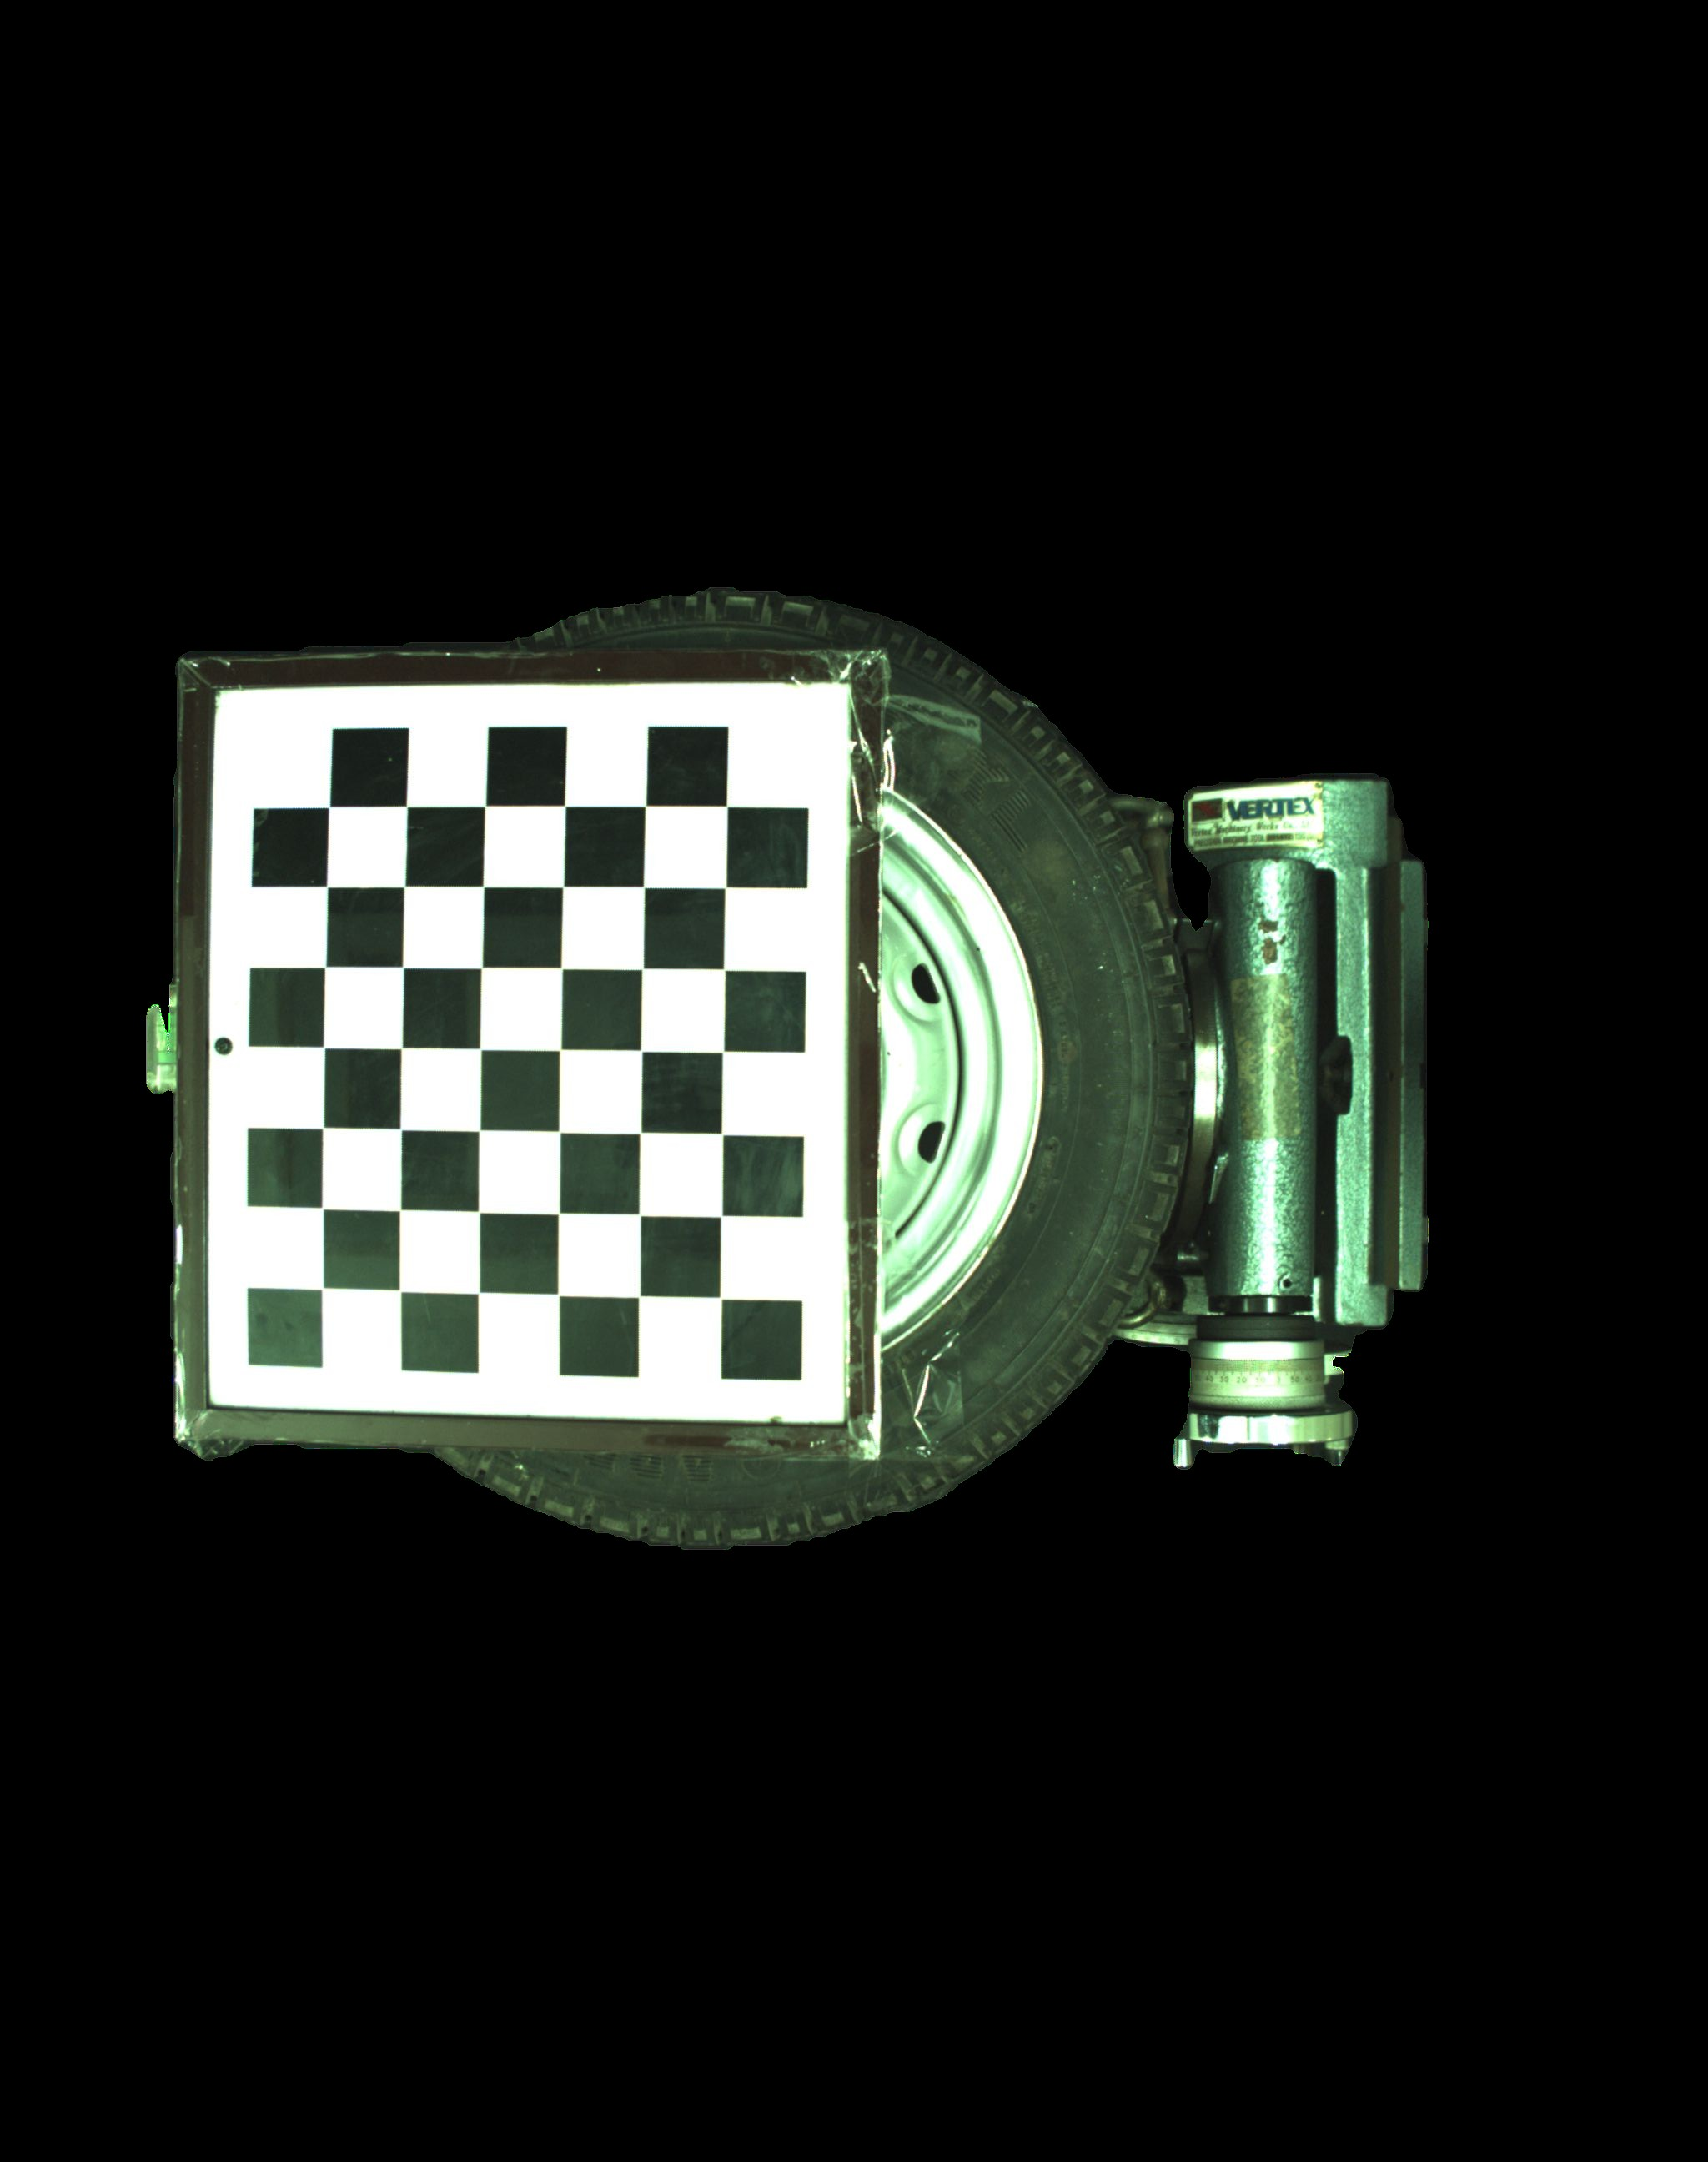
\includegraphics[width=0.24\linewidth]{samples/sample_56/image1.jpg} &
        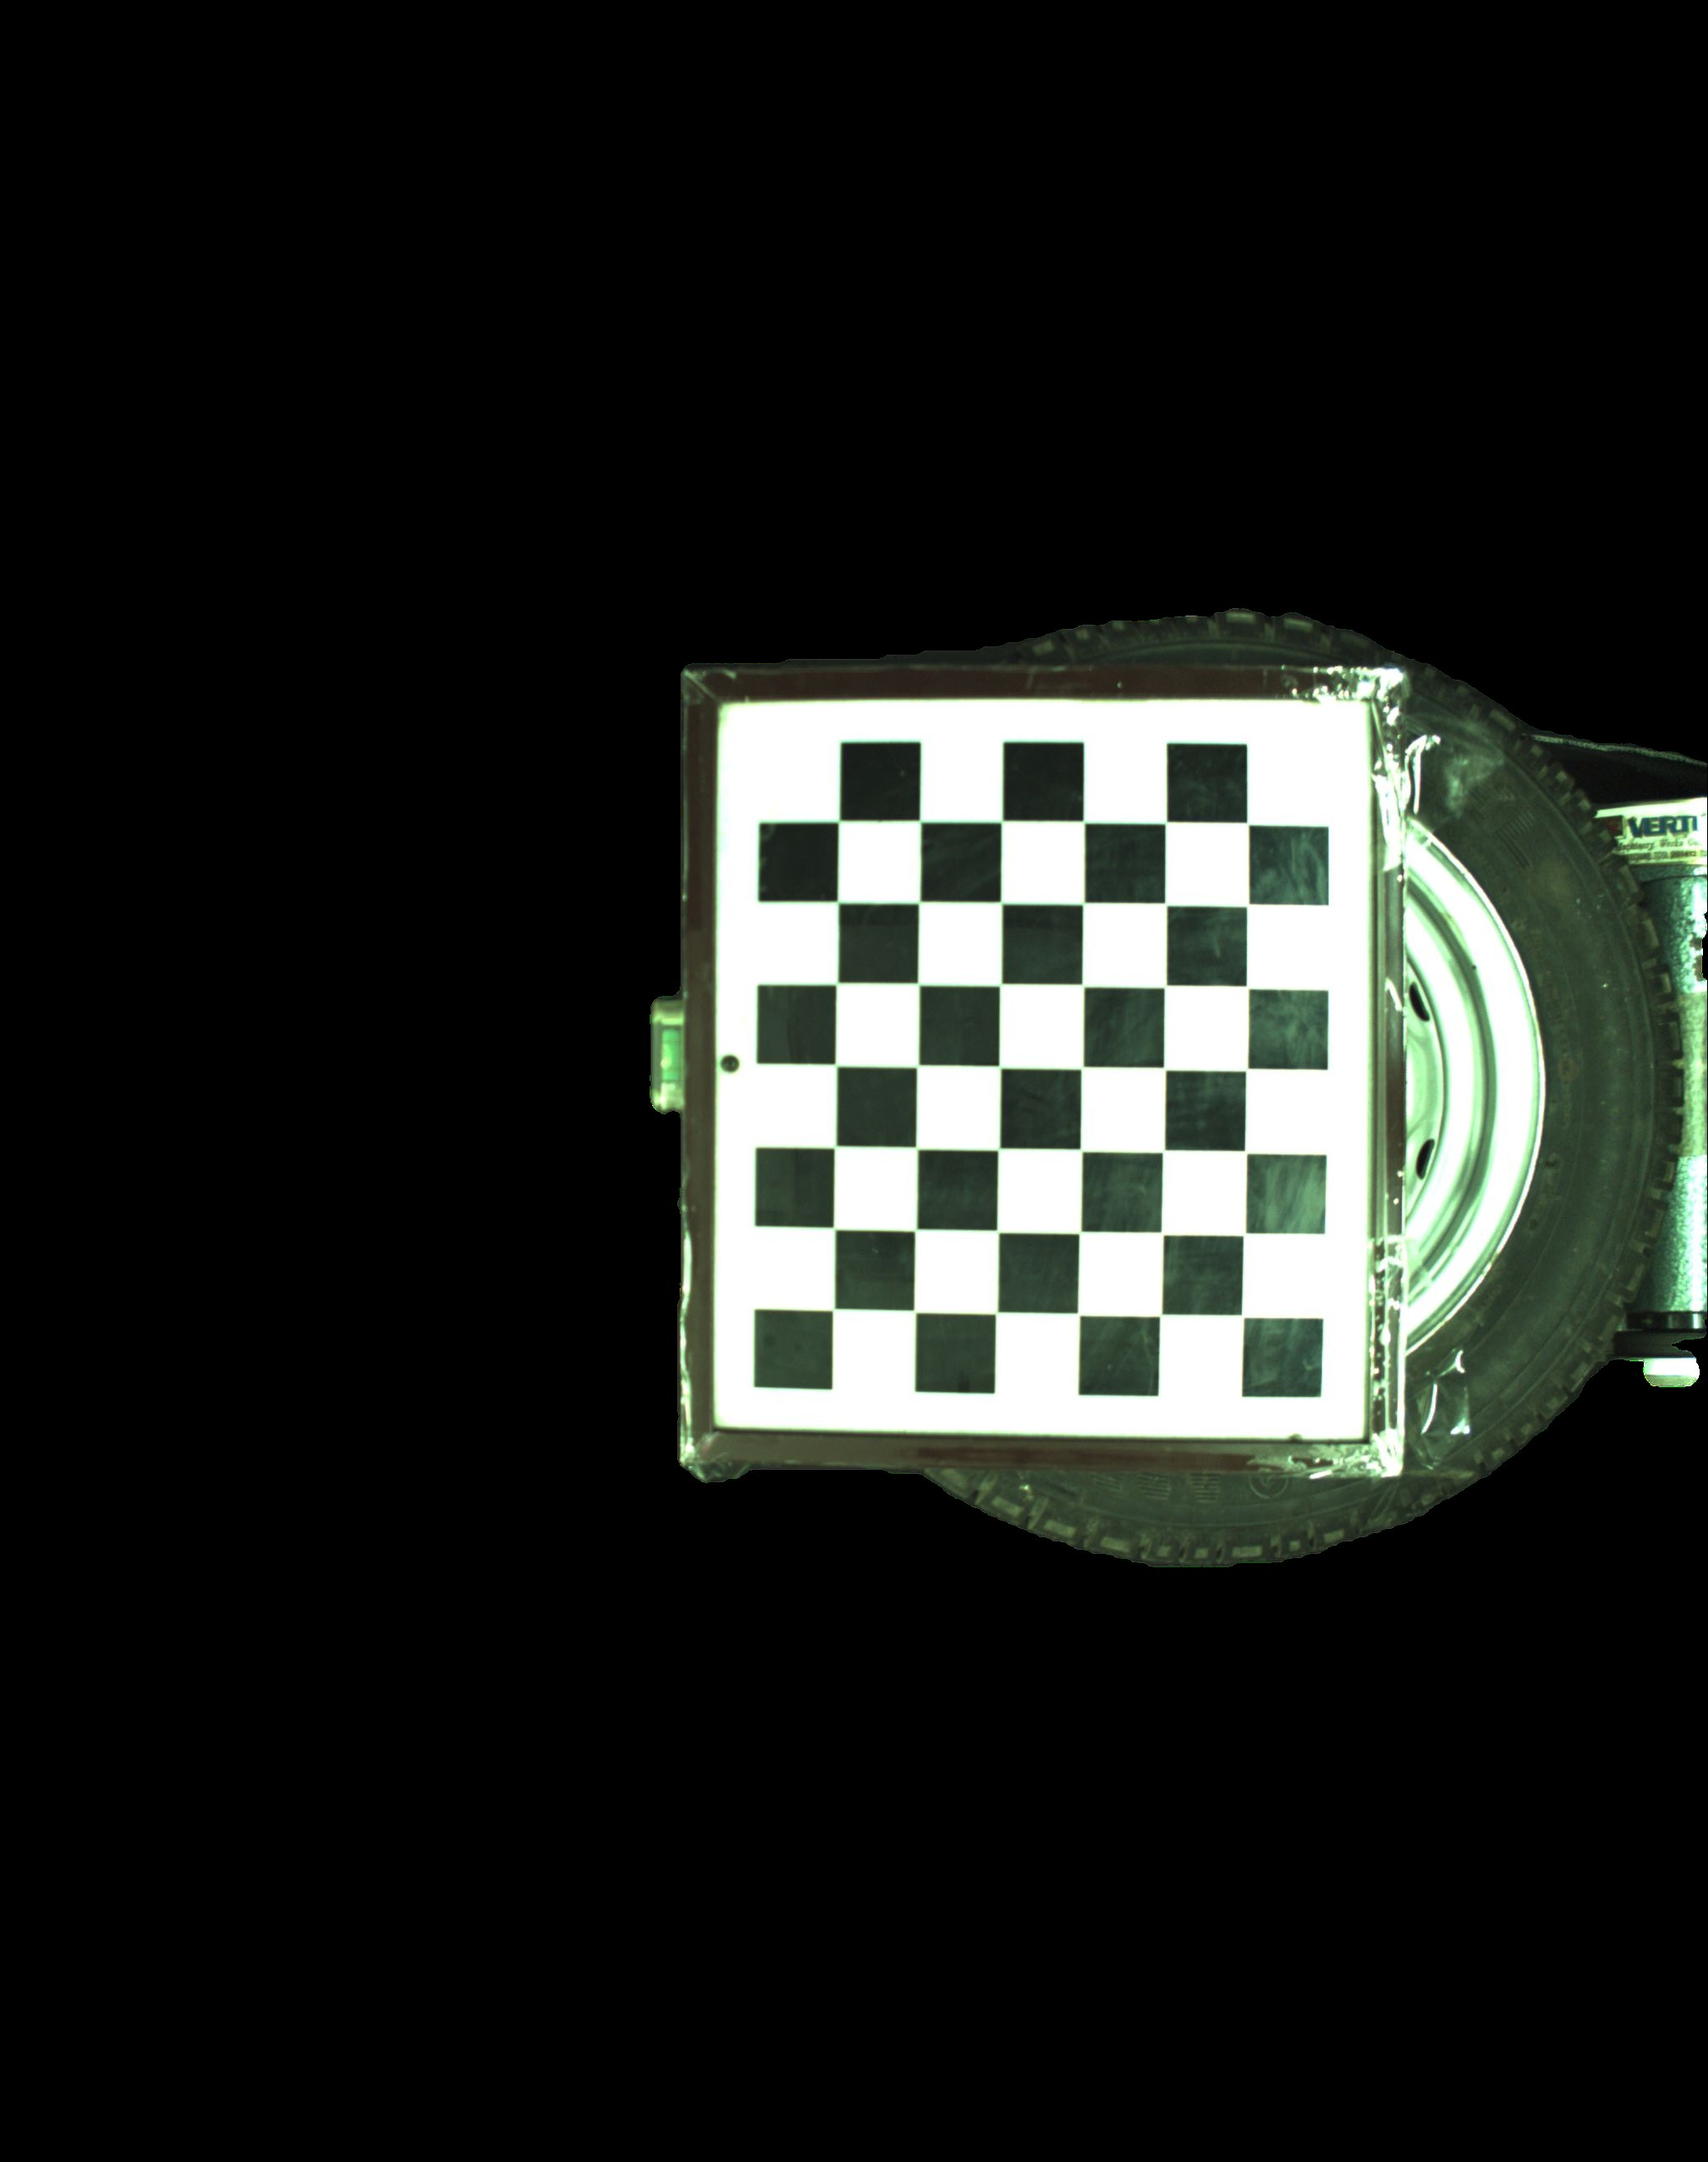
\includegraphics[width=0.24\linewidth]{samples/sample_56/image2.jpg} &
        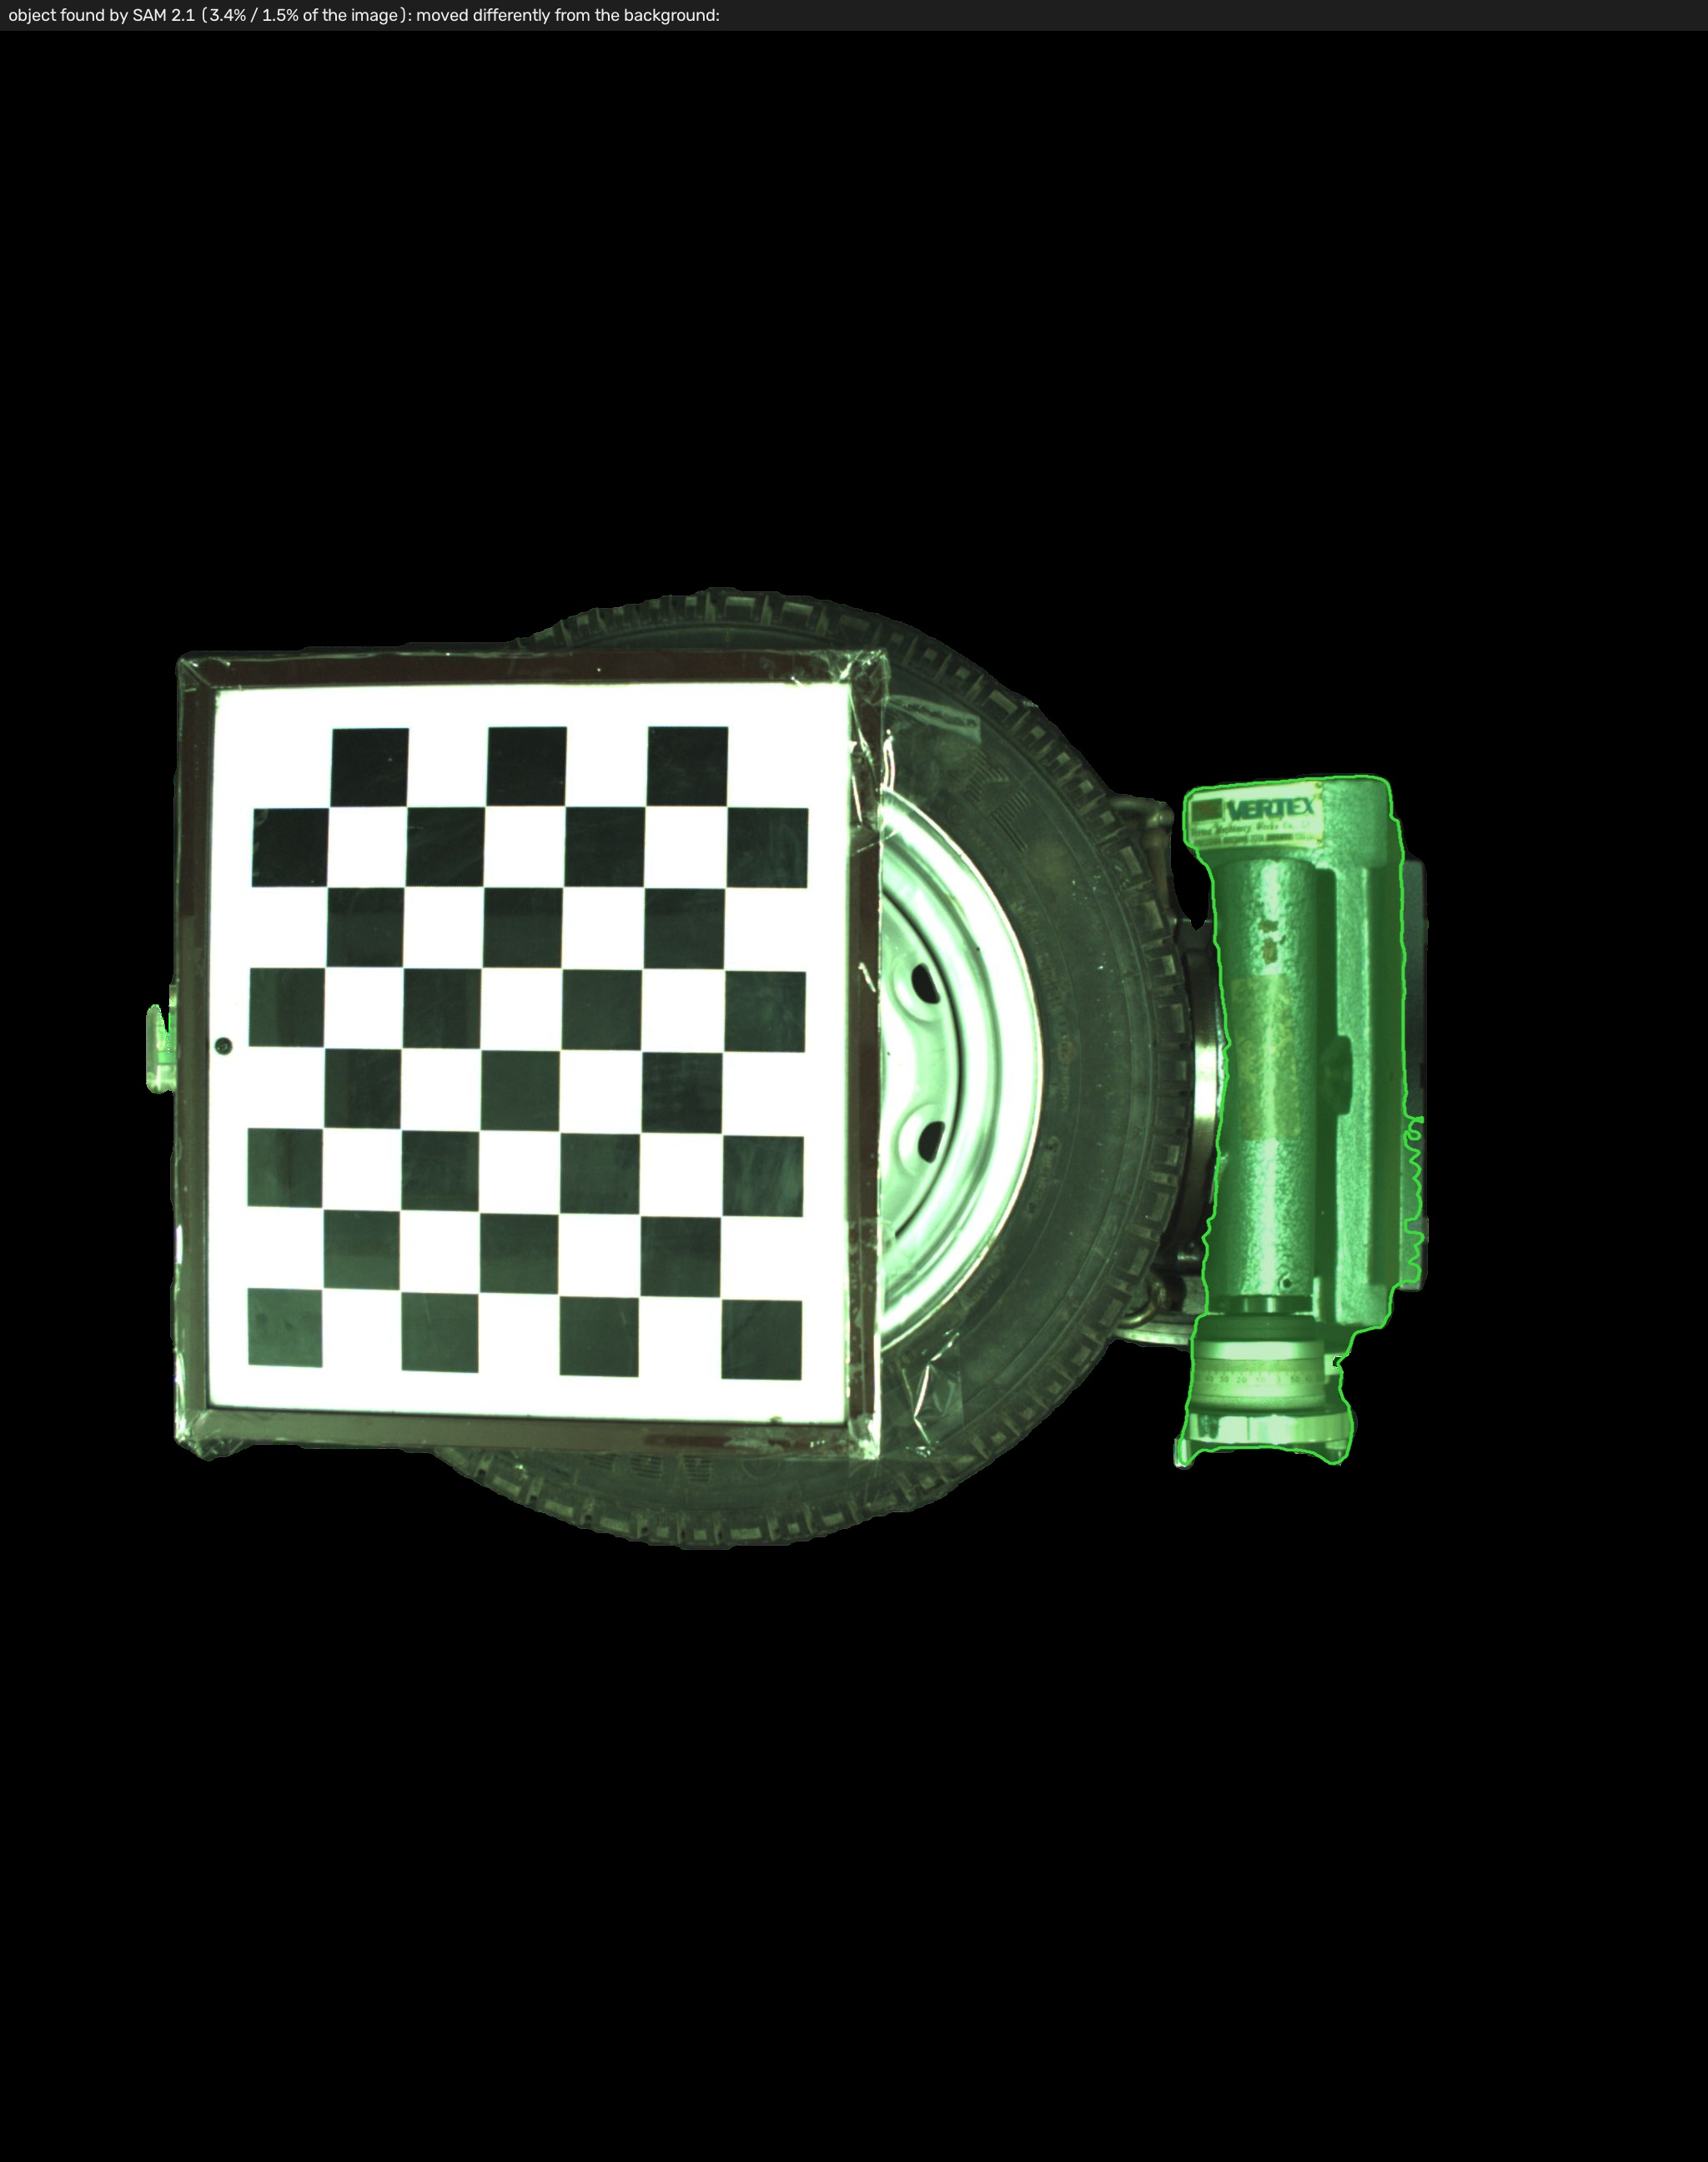
\includegraphics[width=0.24\linewidth]{samples/sample_56/result_mask1.jpg} &
        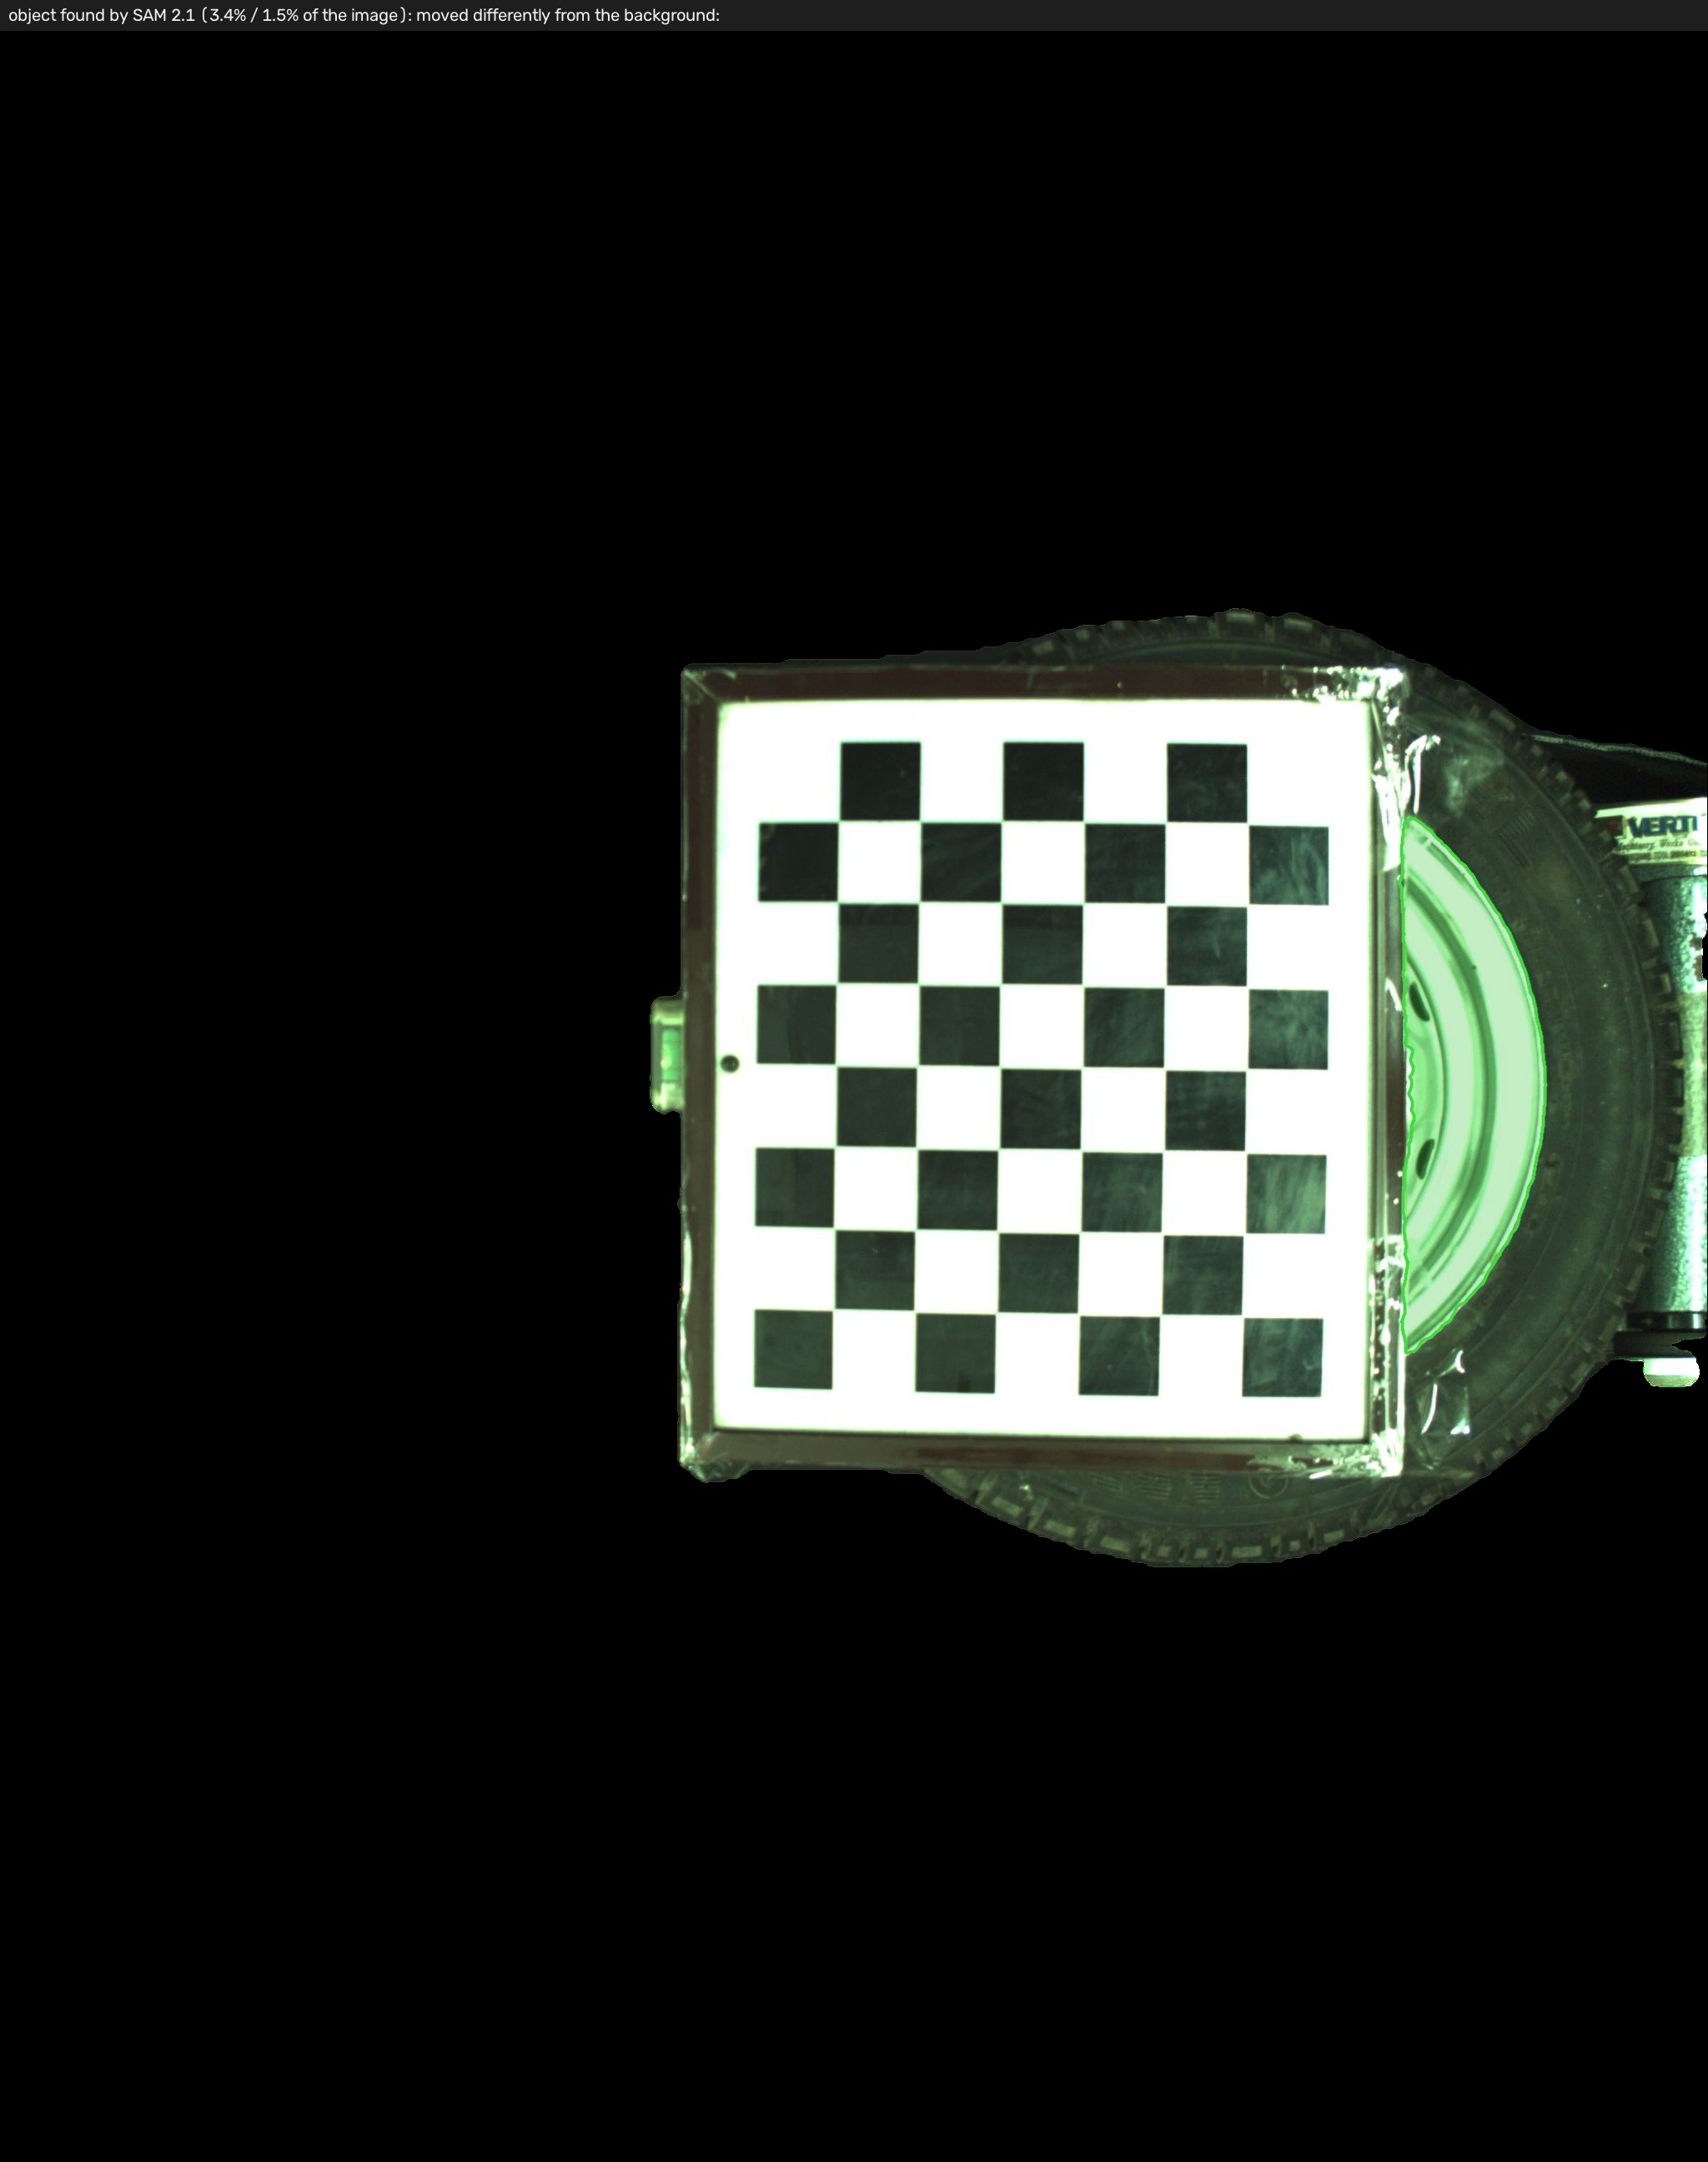
\includegraphics[width=0.24\linewidth]{samples/sample_56/result_mask2.jpg}\\
        image 1 & image 2 & region 1 (green) & region 2 (green)\\[3pt]
        \multicolumn{4}{c}{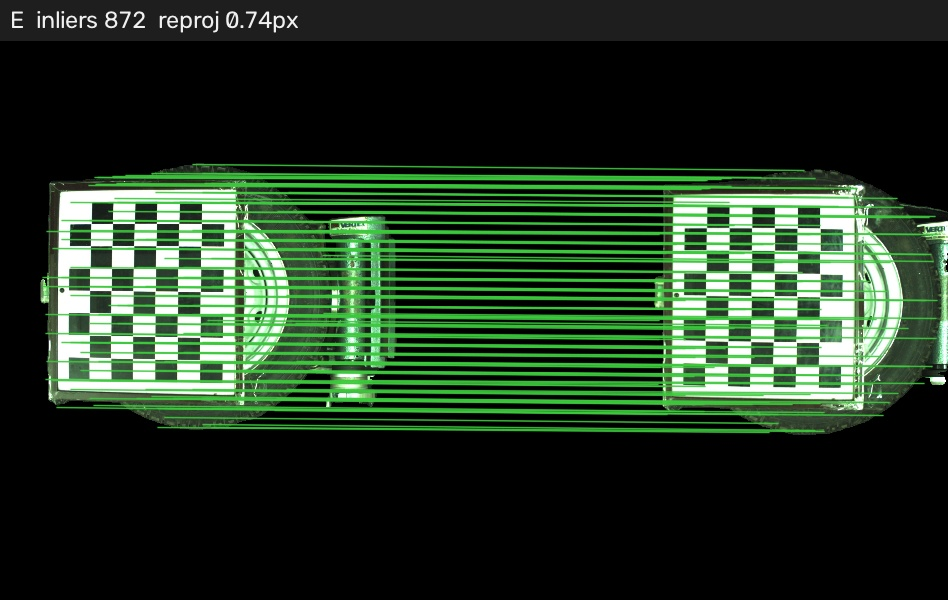
\includegraphics[width=0.62\linewidth]{samples/sample_56/result.jpg}}\\
        \multicolumn{4}{c}{MASt3R inlier correspondences (whole images, after the retry)}
      \end{tabular}
    \end{column}
    \begin{column}{0.42\textwidth}
      \begin{block}{Result (two images only, MASt3R)}
        \scriptsize
        \[\R=\begin{pmatrix}0.99927&0.00124&-0.03810\\-0.00101&0.99998&0.00619\\0.03811&-0.00615&0.99926\end{pmatrix}\]
        \[\tv=(1.000,\,0.014,\,0.006)\ \text{(direction)}\]
        \begin{tabular}{@{}ll@{}}
          Rotation angle & $2.21^\circ$\\
          Rotation axis & $\approx(-0.16,\,-0.99,\,-0.03)$, vertical\\
          Reprojection RMS & 0.74\,px\\
          Model (GRIC) & $E$ (3D)\\
          Inliers / matches & 872 / 873\\
          Focal length & 1779\,px (estimated)\\
          Region & whole images (retry)\\
          Pose time & 15.1\,s\\
          Verdict & \textsc{scene motion only}\\
        \end{tabular}
      \end{block}
      \footnotesize The region finder paired different parts (clamp vs.\ hub), so the pose was recomputed on the whole images. The background is black, so every match lies on the object: the assembly turned by about $2.2^\circ$ about the vertical axis and shifted along $+x$.
    \end{column}
  \end{columns}
\end{frame}

% ------------------------------------------------------------------ instructor's pairs
\begin{frame}{Instructor's test pair A --- given $\K$, all objects move together}
  \begin{columns}[T]
    \begin{column}{0.56\textwidth}
      \centering\scriptsize
      \begin{tabular}{@{}c@{\hspace{3pt}}c@{}}
        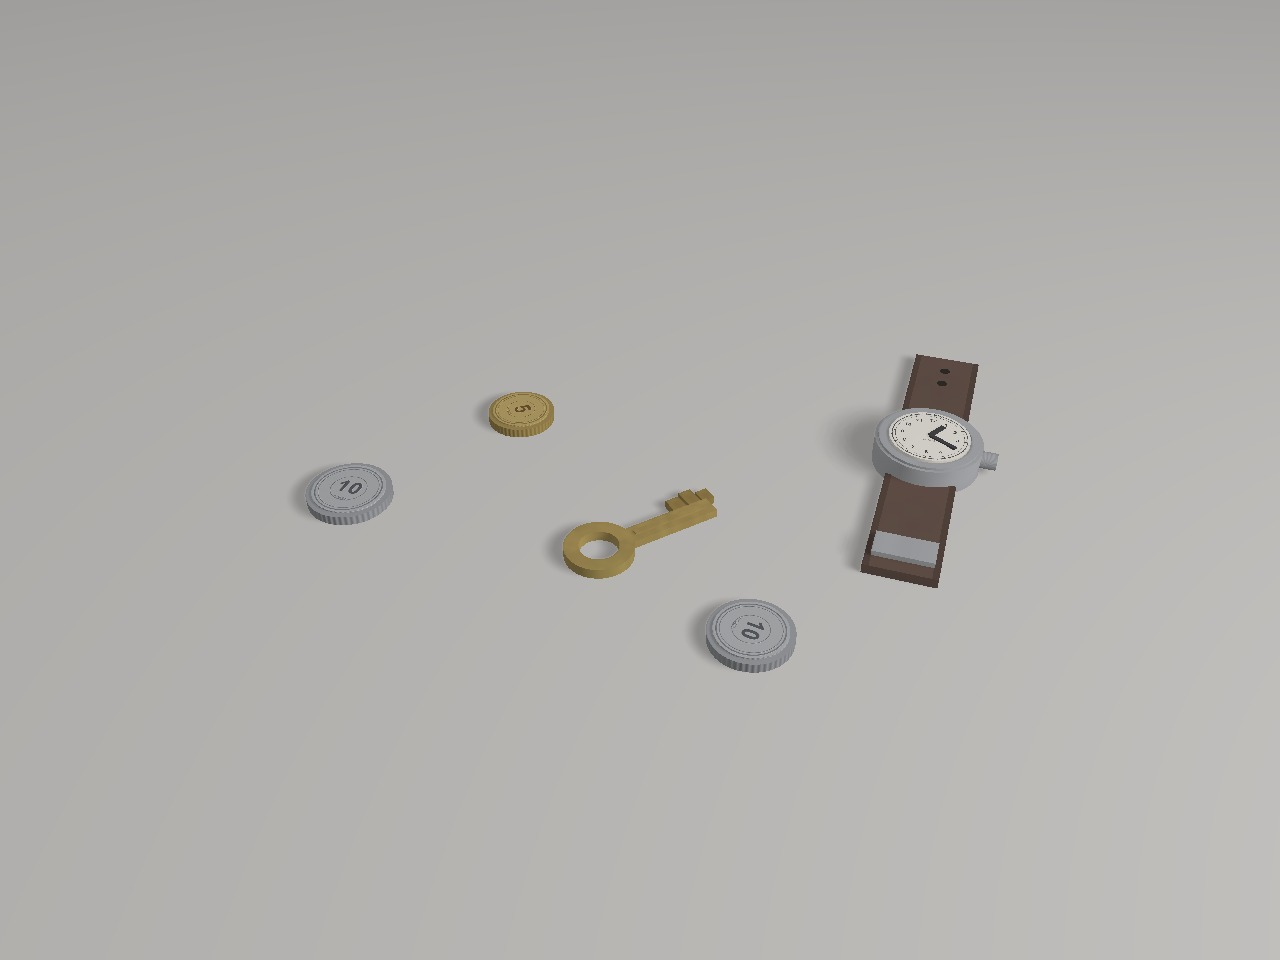
\includegraphics[width=0.49\linewidth]{samples/prof_pairA/pairA_1.jpg} &
        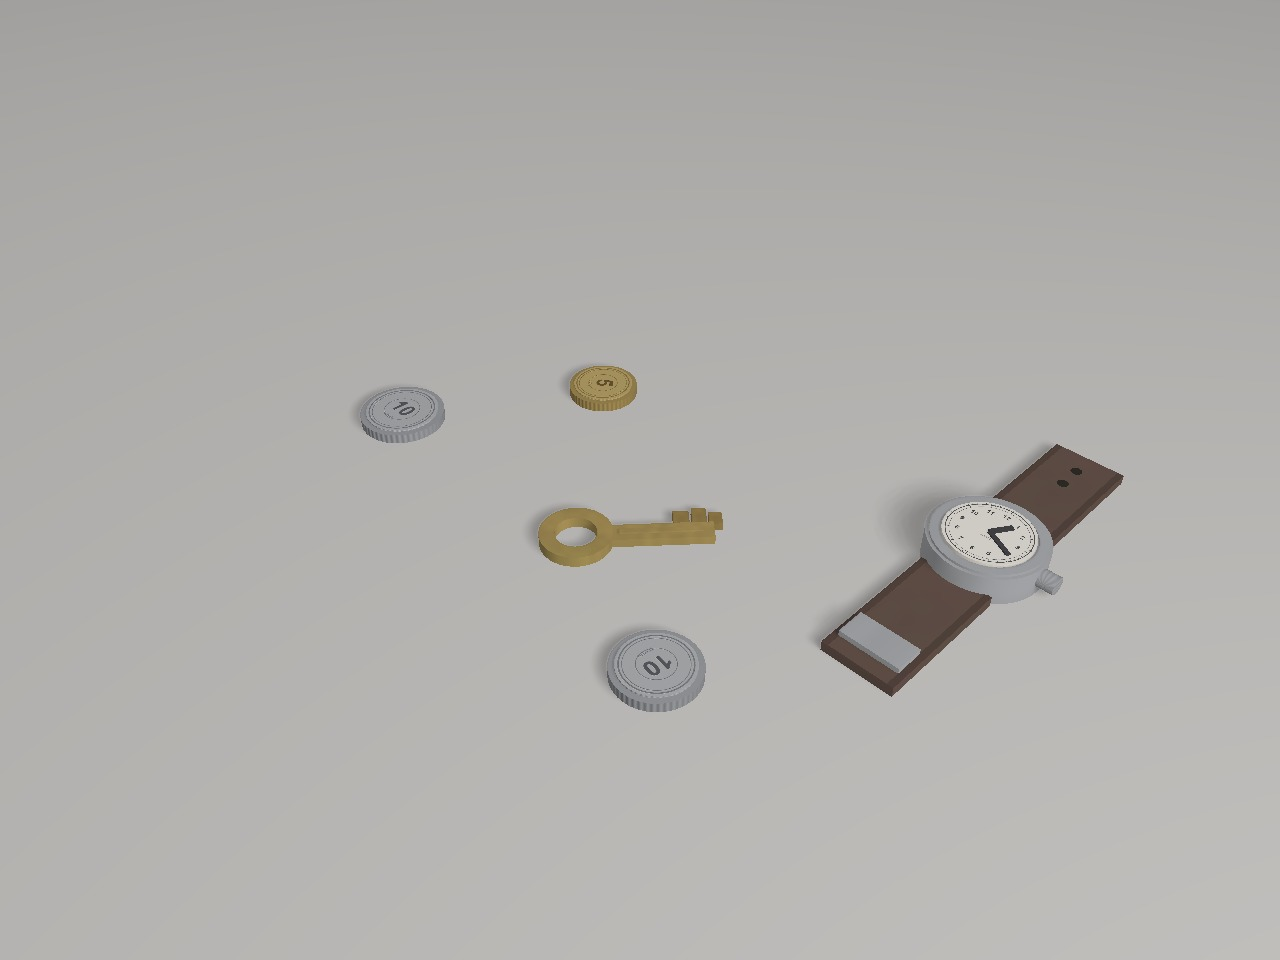
\includegraphics[width=0.49\linewidth]{samples/prof_pairA/pairA_2.jpg}\\
        image 1 & image 2\\[3pt]
        \multicolumn{2}{@{}c@{}}{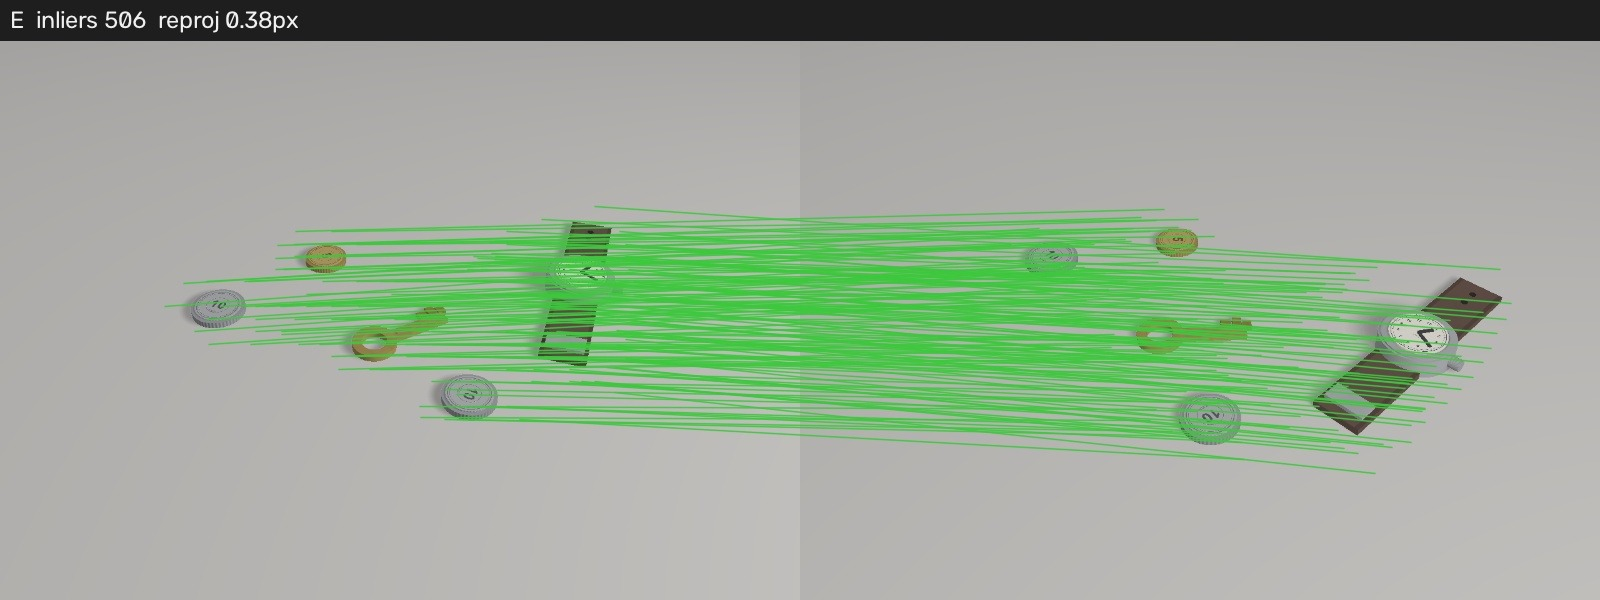
\includegraphics[width=\linewidth]{samples/prof_pairA/pairA_matches.jpg}}\\
        \multicolumn{2}{c}{MASt3R inlier correspondences on the whole images (506 / 513)}
      \end{tabular}
    \end{column}
    \begin{column}{0.42\textwidth}
      \scriptsize
      $\K=\begin{pmatrix}1180&0&640\\0&1180&480\\0&0&1\end{pmatrix}$ (given); one $(\R,\tv)$ for all objects $\Rightarrow$ whole images.
      \begin{block}{Result (two images only, MASt3R)}
        \scriptsize\setlength{\arraycolsep}{3pt}
        \[\R=\begin{pmatrix}0.8906&-0.2852&0.3541\\0.2848&0.9570&0.0545\\-0.3545&0.0524&0.9336\end{pmatrix}\]
        \[\tv=(-0.988,\,-0.152,\,0.020)\ \text{(direction)}\]
        \begin{tabular}{@{}ll@{}}
          Rotation angle & $27.05^\circ$\\
          Rotation axis & $(-0.002,\,0.779,\,0.627)$\\
          Roll / pitch / yaw & $3.21^\circ$ / $20.76^\circ$ / $17.73^\circ$\\
          Model (GRIC) & $E$ (3D)\\
          Inliers / matches & 506 / 513\\
          Reprojection RMS & 0.38\,px\\
          Pose time & 16.8\,s\\
        \end{tabular}
      \end{block}
      \footnotesize The rotation axis lies within $1.6^\circ$ of the table normal $(0.032,\,0.774,\,0.633)$: the objects were turned together by $27^\circ$ about the table normal.
    \end{column}
  \end{columns}
\end{frame}

\begin{frame}{Instructor's test pair C --- same $\K$, all objects move together}
  \begin{columns}[T]
    \begin{column}{0.56\textwidth}
      \centering\scriptsize
      \begin{tabular}{@{}c@{\hspace{3pt}}c@{}}
        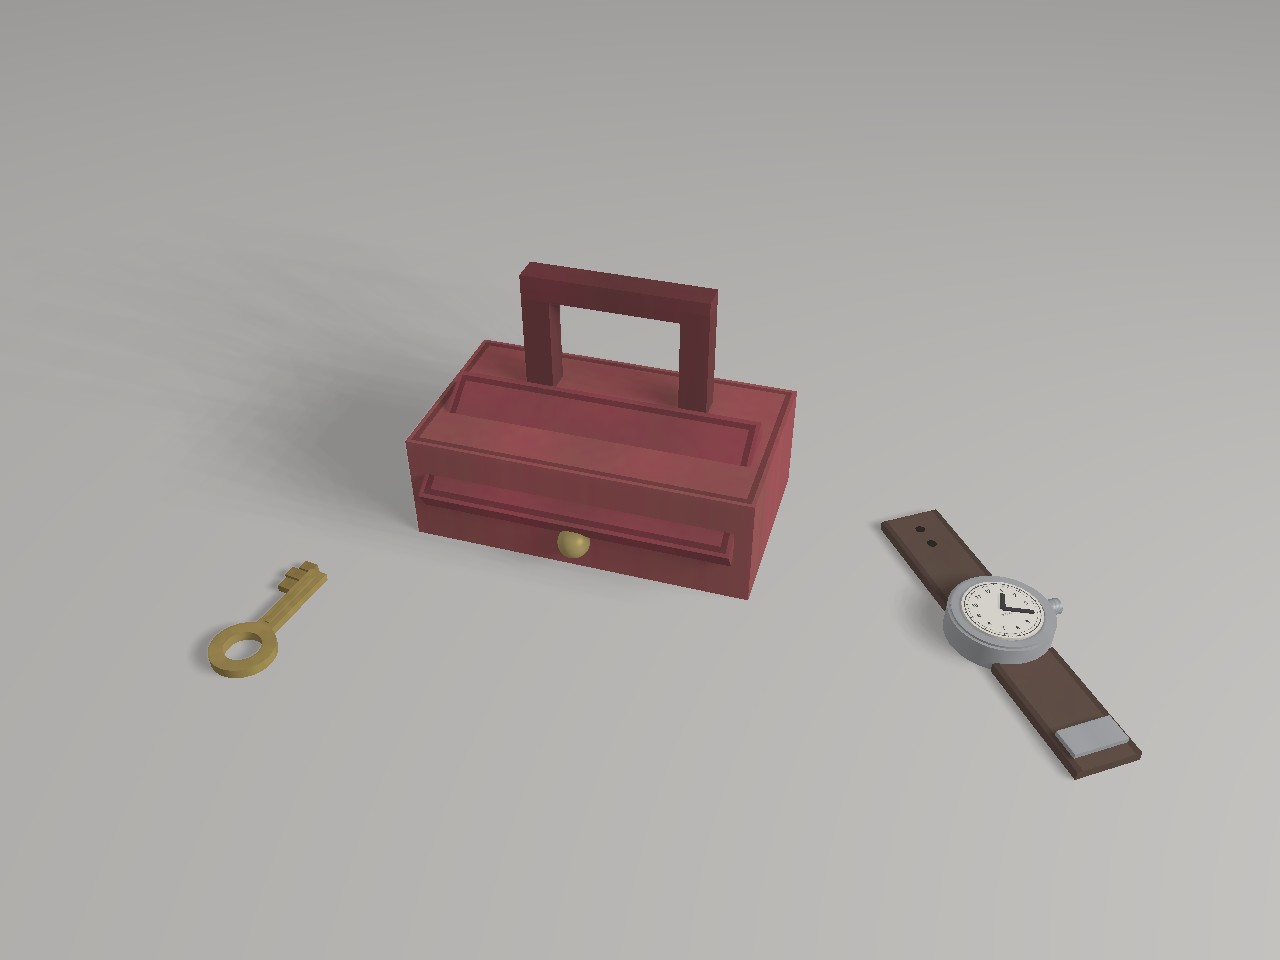
\includegraphics[width=0.49\linewidth]{samples/prof_pairC/pairC_1.jpg} &
        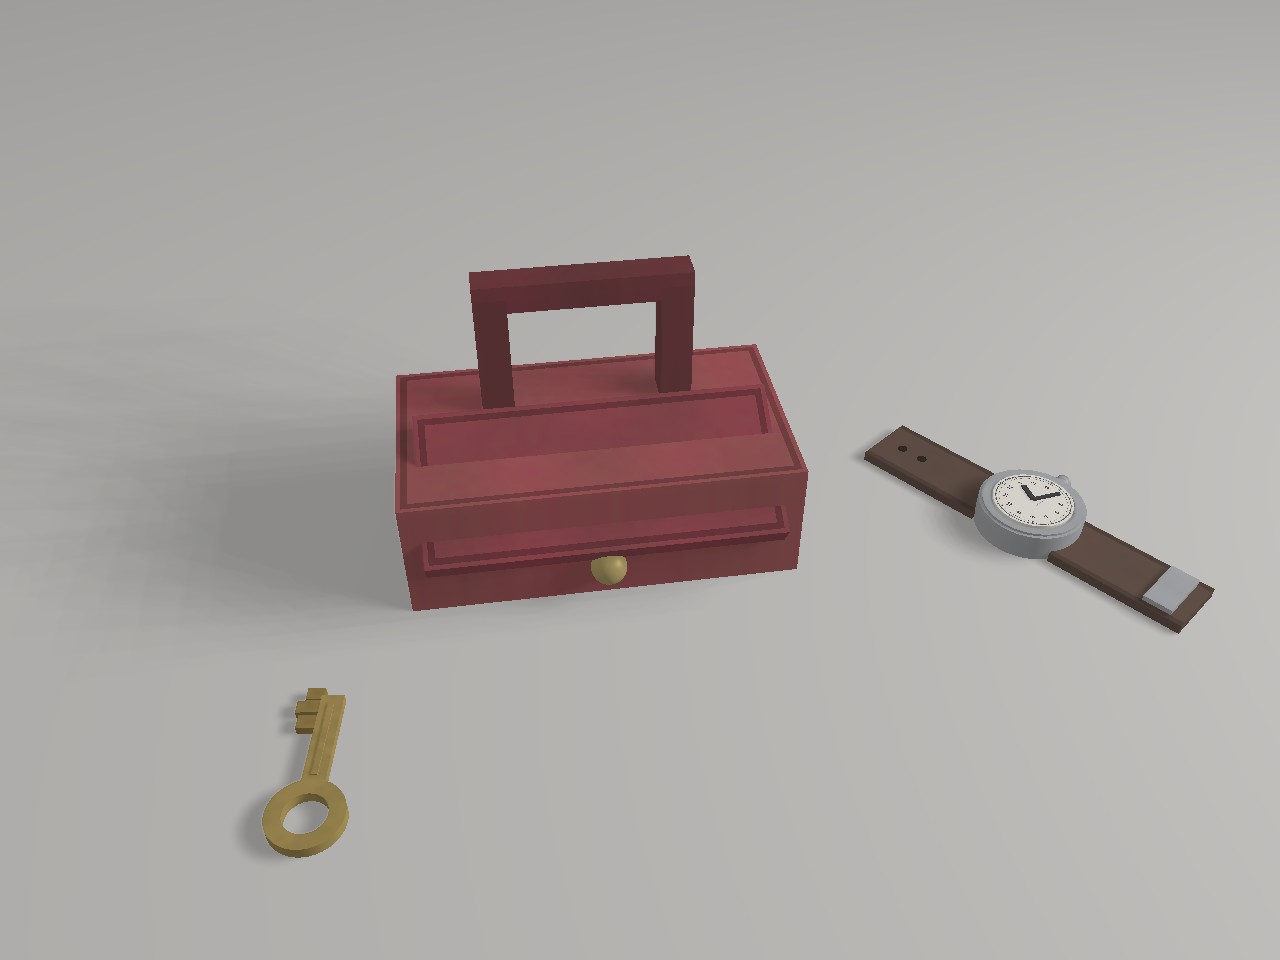
\includegraphics[width=0.49\linewidth]{samples/prof_pairC/pairC_2.jpg}\\
        image 1 & image 2\\[3pt]
        \multicolumn{2}{@{}c@{}}{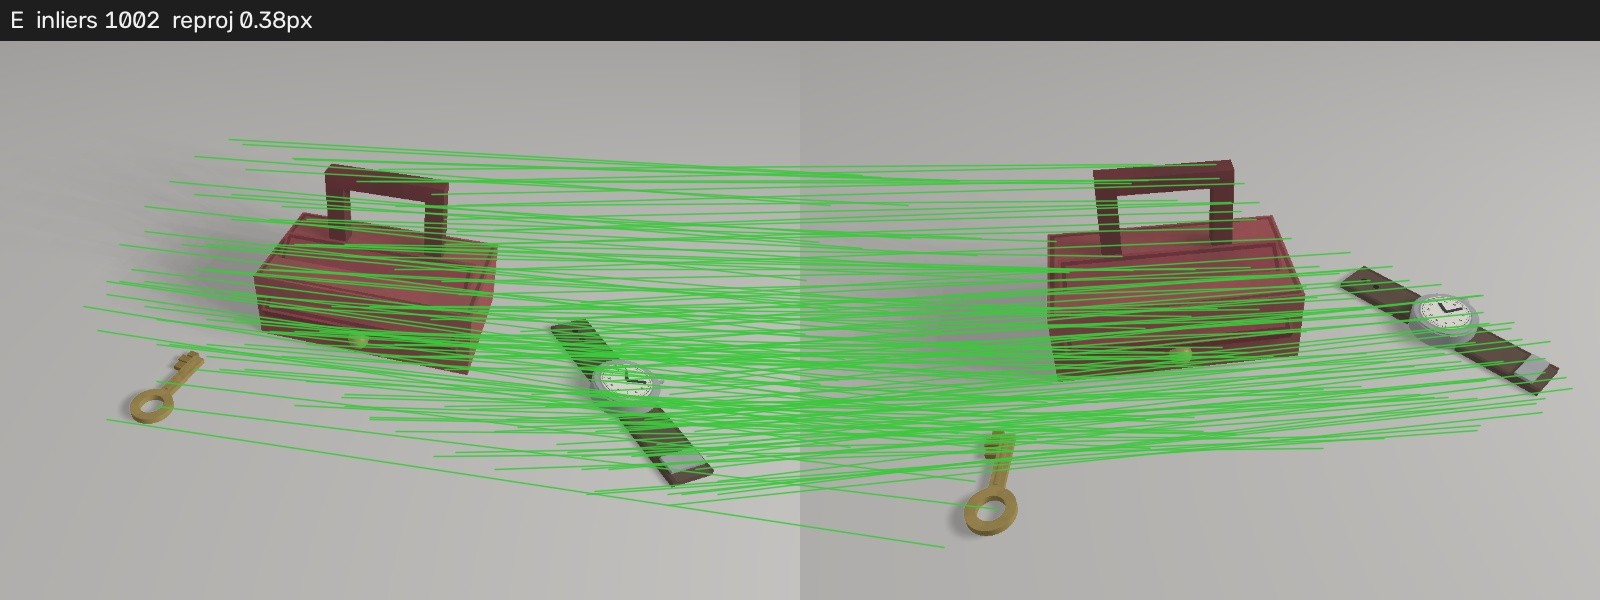
\includegraphics[width=\linewidth]{samples/prof_pairC/pairC_matches.jpg}}\\
        \multicolumn{2}{c}{MASt3R inlier correspondences on the whole images (1002 / 1032)}
      \end{tabular}
    \end{column}
    \begin{column}{0.42\textwidth}
      \scriptsize
      $\K=\begin{pmatrix}1180&0&640\\0&1180&480\\0&0&1\end{pmatrix}$ (given); one $(\R,\tv)$ for all objects $\Rightarrow$ whole images.
      \begin{block}{Result (two images only, MASt3R)}
        \scriptsize\setlength{\arraycolsep}{3pt}
        \[\R=\begin{pmatrix}0.9013&0.2700&-0.3389\\-0.2820&0.9593&0.0141\\0.3289&0.0829&0.9407\end{pmatrix}\]
        \[\tv=(0.995,\,-0.042,\,-0.089)\ \text{(direction)}\]
        \begin{tabular}{@{}ll@{}}
          Rotation angle & $25.76^\circ$\\
          Rotation axis & $(0.079,\,-0.768,\,-0.635)$\\
          Roll / pitch / yaw & $5.03^\circ$ / $-19.20^\circ$ / $-17.38^\circ$\\
          Model (GRIC) & $E$ (3D)\\
          Inliers / matches & 1002 / 1032\\
          Reprojection RMS & 0.38\,px\\
          Pose time & 21.2\,s\\
        \end{tabular}
      \end{block}
      \footnotesize The rotation axis lies within $6.2^\circ$ of the table normal $(0.023,\,0.745,\,0.666)$, opposite sign: turned together by $25.8^\circ$, the other way from pair A.
    \end{column}
  \end{columns}
\end{frame}

% ------------------------------------------------------------------ references
\begin{frame}{References}
  \begin{columns}[T]
    \begin{column}{0.49\textwidth}
      \tiny
      \begin{enumerate}
        \item[{[1]}] R.~Hartley, A.~Zisserman, \emph{Multiple View Geometry in Computer Vision}, 2nd ed., Cambridge Univ.\ Press, 2004.
        \item[{[2]}] E.~Weiszfeld, ``Sur le point pour lequel la somme des distances de $n$ points donn\'es est minimum,'' \emph{T\^ohoku Math.\ J.}, 1937.
        \item[{[3]}] V.~Leroy, Y.~Cabon, J.~Revaud, ``Grounding image matching in 3D with MASt3R,'' \emph{ECCV}, 2024.
        \item[{[4]}] S.~Wang, V.~Leroy, Y.~Cabon, B.~Chidlovskii, J.~Revaud, ``DUSt3R: Geometric 3D vision made easy,'' \emph{CVPR}, 2024.
        \item[{[5]}] N.~Ravi \emph{et al.}, ``SAM 2: Segment anything in images and videos,'' arXiv:2408.00714, 2024.
        \item[{[6]}] C.~Ryali \emph{et al.}, ``Hiera: A hierarchical vision transformer without the bells-and-whistles,'' \emph{ICML}, 2023.
        \item[{[7]}] D.~Barath, J.~Noskova, M.~Ivashechkin, J.~Matas, ``MAGSAC++, a fast, reliable and accurate robust estimator,'' \emph{CVPR}, 2020.
        \item[{[8]}] M.~Irani, P.~Anandan, ``A unified approach to moving object detection in 2D and 3D scenes,'' \emph{IEEE TPAMI}, 1998.
        \item[{[9]}] J.~P.~Lewis, ``Fast normalized cross-correlation,'' \emph{Vision Interface}, 1995.
        \item[{[10]}] D.~G.~Lowe, ``Distinctive image features from scale-invariant keypoints,'' \emph{IJCV}, 2004.
        \item[{[11]}] G.~Potje \emph{et al.}, ``XFeat: Accelerated features for lightweight image matching,'' \emph{CVPR}, 2024.
        \item[{[12]}] P.~Lindenberger, P.-E.~Sarlin, M.~Pollefeys, ``LightGlue: Local feature matching at light speed,'' \emph{ICCV}, 2023.
      \end{enumerate}
    \end{column}
    \begin{column}{0.49\textwidth}
      \tiny
      \begin{enumerate}
        \item[{[13]}] J.~Sun, Z.~Shen, Y.~Wang, H.~Bao, X.~Zhou, ``LoFTR: Detector-free local feature matching with transformers,'' \emph{CVPR}, 2021.
        \item[{[14]}] D.~Nist\'er, ``An efficient solution to the five-point relative pose problem,'' \emph{IEEE TPAMI}, 2004.
        \item[{[15]}] M.~A.~Fischler, R.~C.~Bolles, ``Random sample consensus,'' \emph{Comm.\ ACM}, 1981.
        \item[{[16]}] P.~H.~S.~Torr, ``Geometric motion segmentation and model selection,'' \emph{Phil.\ Trans.\ Royal Society A}, 1998.
        \item[{[17]}] E.~Malis, M.~Vargas, ``Deeper understanding of the homography decomposition for vision-based control,'' INRIA RR-6303, 2007.
        \item[{[18]}] K.~Levenberg, ``A method for the solution of certain non-linear problems in least squares,'' \emph{Q.\ Appl.\ Math.}, 1944.
        \item[{[19]}] D.~W.~Marquardt, ``An algorithm for least-squares estimation of nonlinear parameters,'' \emph{SIAM J.\ Appl.\ Math.}, 1963.
        \item[{[20]}] J.~Sturm \emph{et al.}, ``A benchmark for the evaluation of RGB-D SLAM systems,'' \emph{IROS}, 2012.
        \item[{[21]}] A.~Ahmadyan \emph{et al.}, ``Objectron: A large scale dataset of object-centric videos in the wild with pose annotations,'' \emph{CVPR}, 2021.
        \item[{[22]}] J.~Reizenstein \emph{et al.}, ``Common Objects in 3D,'' \emph{ICCV}, 2021.
        \item[{[23]}] X.~Yu \emph{et al.}, ``MVImgNet: A large-scale dataset of multi-view images,'' \emph{CVPR}, 2023.
        \item[{[24]}] P.-E.~Sarlin \emph{et al.}, ``SuperGlue: Learning feature matching with graph neural networks,'' \emph{CVPR}, 2020.
        \item[{[25]}] J.~J.~Mor\'e, ``The Levenberg--Marquardt algorithm: implementation and theory,'' \emph{Numerical Analysis}, LNM 630, Springer, 1978.
        \item[{[26]}] Y.~Ma, S.~Soatto, J.~Ko\v{s}eck\'a, S.~S.~Sastry, \emph{An Invitation to 3-D Vision}, Springer, 2004.
      \end{enumerate}
    \end{column}
  \end{columns}
\end{frame}

% ------------------------------------------------------------------ 16 thanks
\begin{frame}[plain]
  \centering
  \vspace*{2.2cm}
  {\usebeamercolor[fg]{structure}\Huge\bfseries Thank you\par}
  \vspace{0.6cm}
  {\large Questions?\par}
  \vspace{1.2cm}
  {\small Sai Svanik Chiramana (ME23B195) \qquad Sathwik Chanduluri (ME23B238) \qquad Group 3\par}
\end{frame}

\end{document}
